\documentclass[handout]{beamer}
%\documentclass{beamer}


% MAKEN VAN BACKGROUND ETC.
\mode<presentation> {
 \usetheme{CambridgeUS} %stijl van de presentatie
  \setbeamercovered{transparent}
    \usecolortheme{beaver} %kleurpatroon
}

% INLADEN VAN PACKAGES%


\usepackage{psboxit}
\usepackage{fancybox}
\usepackage{colordvi}
\usepackage{epsfig}
\usepackage{url}
\usepackage{palatino}
\usepackage[dutch]{babel}
\usepackage[latin1]{inputenc} 
\usepackage{times}
\usepackage[T1]{fontenc}
\usepackage{graphicx}
\usepackage{subfigure}
\newtheorem{eigenschap}[theorem]{Eigenschap}
\usepackage{amssymb,amsmath}
\usepackage{pgflibraryarrows}
\usepackage{tikz}
\usepackage[absolute,overlay]{textpos}
\usepackage{colortbl}
\usepackage{multimedia}

\usepackage{hyperref}
\hypersetup{
    colorlinks,%
    citecolor=black,%
    filecolor=black,%
    linkcolor=black,%
    urlcolor=blue     % can put red here to visualize the links
}

%\DeclareGraphicsExtensions{.pdf,.png,.gif,.jpg}

\setcounter{tocdepth}{1}

%-------Textpos setup and grid command-----

\setlength{\TPHorizModule}{\the\paperwidth}  %defines unit length for textpos

\newcommand<>{\makegrid}[0]{
\begin{textblock}{1}(0,0) % width of block, origin at top left corner of page
\uncover#1{
\begin{tikzpicture}[color=blue!40!black!30,very thin]
\draw[step=.5cm,draw opacity=.5] (0,0) grid
(\the\paperwidth,\the\paperheight);
\foreach \x in {1,2,...,12}
   \draw[text=black] (\x,.15) node {\footnotesize \x};
\foreach \y in {1,2,...,9}
   \draw[text=black] (.2,\y) node {\footnotesize \y};
\end{tikzpicture}  }
\end{textblock}
}

\newcommand{\btx}{\begin{textblock}{1}(0,0)}
\newcommand{\etx}{\end{textblock}}

% INLADEN VAN MACRO-FILE
 %% file: rrmacros2e.tex = Rob Rutten's standard LaTeX macros
%% last: Mar  9 2006 
%% site: ~/rr/tex/macros
%% note: convert to rmacros2e.tex with bindip/convertmacros2e

%%%%%%%%%%%%%%%%%%%%%%%%%%%%%%%%%%%%%%%%%%%%%%%%%%%%%%%%% BIBTEX EXPLANATION
%% Use BibTeX with the proper JOURNAL.STY, BIB.STY and BIB.BST style files.
%% The required statement combinations sit in template files:
%%    RRPAPER.TPL, AAPAPER.TPL, APJPAPER.TPL, ESAPROC.TPL, KLUWER.TPL,
%%    SWANSONG.TPL, PASP.TPL etc.,  
%% linked to directory /rrtex/templates
%% My RJR-typed -.BIB files are linked to /rrtex/bibfiles/rjr/bib.
%% My ADS-copied -.BIB files are linked to /rrtex/bibfiles/ads/bib.
%% Journal abbreviations are specified in AAJOUR.BIB (A&A, APJ format) and
%%   in JOURNALS.BIB (classical longer format), both in /rrtex/styles.
%%   The ADS abbreviations are redefined below (also two formats).
%% To use bibtex use script rrbibtex (in ~rutten/bin).
%%
%% Cites:   \cite*{Rutten1990a}                        }      
%%               ==>  Rutten (1990)                    } for in-text
%%          \cite*{Gurtovenko+Kostik+Rutten1990b}      } references
%%               ==>  Gurtovenko et al. (1990)        }
%%          \cite{Rutten1990a}                       }
%%               ==>  Rutten 1990                    } for between (...)
%%          \cite{Gurtovenko+Kostik+Rutten1990b}     } references
%%               ==>  Gurtovenko et al. 1990          }
%%          (Rutten 1990a, 1990b)
%%                    \nocite{Rutten1990c}  
%%                    \nocite{Rutten1990f}
%%          NB: \nocite*{..} makes Bibtex produce ALL bibliography entries
%%          NB: Bibtex may mix up the order, putting a later paper
%%              before an earlier one even in the same journal, becauses it
%%              alphabetizes on title after authors.  If it bothers you
%%              then correct the final -.BBL file, or fix the problem
%%              by adding fake digits to TITLE fields in .BIB files 
%%              (see Jo Bruls' README_order with my -.BIB files).
%%
%% Full citations for publication lists and PRINTBIB:
%%              \fullreferences (adds full titles and end pages)
%% 
%% References:
%%          - RRBIB: \section*{References} \references 
%%          - FULLBIB: \section*{References} \fullreferences
%%          - AABIB: no section header, \aareferences
%%          - APJBIB: no section header, \apjreferences
%%          - KLUWBIB: no section header, \references
%%          - ESA: no BIB.STY, section header ESAPROC.TPL, \esareferences
%%          - set \parsep=0ex to delete blank lines between references
%%          - execute latex, rrbibtex, latex twice
%%          - for email/ftp transfer: comment \references statement out and
%%            merge the -.BBL file there instead, or ftp that as well.
%%            Also ftp or insert this macro file, and email/ftp xxxBIB.STY.
%%
%% Database printout: ps files under /rrtex/bibfiles
%%
%% ADS: As of July 1996 I use ADS entries.  I  pull XXX.BIB files over
%%      from ADS and also XXX.ABS files with the corresponding abstracts.  
%%      They sit in /rrtex/bibfiles/ads/bib and /rrtex/bibfiles/ads/abs.
%%      Script RRBIBTEX copies all the XXX.BIB files to a short-lived
%%      file /scratch/strknd/rutten/adsfiles.bib that is searched by BibTeX 
%%      (appropriate BibTeX path in my .login) from script RRBIBTEX.
%%      BibTeX may complain about repeated ADS entries; don't bother.
%% NB: don't refer to the same paper with both its ADS XXX.BIB label 
%%     and its old bibfile label - or you get that reference twice.
%%     Check the resulting reference list for such duplicates.
%%%%%%%%%%%%%%%%%%%%%%%%%%%%%%%%%%%%%%%%%%%%%%%%%%%%%%%%%%%%%%%%%%%%%%%%%%%%%

%% ADS character defs
\def\amp{\&}

%% ADS journal abbreviations: long and short versions, also in RJR.BIB
\newcount\longrefs
\def\aap{\ifnum\longrefs=1 {Astron.\ Astrophys.}\else 
                           {A\hbox{\rm \&}A}\fi}
\def\aapr{\ifnum\longrefs=1 {Astron.\ Astrophys.\ Rev.}\else 
                            {A\hbox{\rm \&}AR}\fi}
\def\aaps{\ifnum\longrefs=1 {Astron.\ Astrophys.\ Suppl.}\else 
                            {A\hbox{\rm \&}A Suppl.}\fi}
\def\aj{\ifnum\longrefs=1 {Astron.\ J.}\else 
                          {AJ}\fi} 
\def\ao{\ifnum\longrefs=1 {Applied Optics}\else 
                           {Appl.\ Opt.}\fi} 
\def\aspcs{\ifnum\longrefs=1 {Astron.\ Soc.\ Pacific Conf. Series}\else 
                           {ASP Conf.\ Ser.}\fi} 
\def\apj{\ifnum\longrefs=1 {Astrophys.\ J.}\else 
                           {ApJ}\fi} 
\def\apjl{\ifnum\longrefs=1 {Astrophys.\ J. Lett.}\else 
                            {ApJ}\fi} 
\def\aplett{\ifnum\longrefs=1 {Astrophys.\ J. Lett.}\else 
                            {ApJ}\fi} 
\def\apjs{\ifnum\longrefs=1 {Astrophys.\ J. Suppl.}\else 
                            {ApJS}\fi}
\def\apss{\ifnum\longrefs=1 {Astrophys.\ and Space Science}\else 
                            {Astrophys.\ Space Sci.}\fi}
\def\araa{\ifnum\longrefs=1 {Ann.\ Rev.\ Astron.\ Astrophys.}\else 
                            {ARA\hbox{\rm \&}A}\fi}
\def\azh{\ifnum\longrefs=1 {Astronomicheskii Zhurnal}\else 
                            {Astron.\ Zhur.}\fi}
\def\baas{\ifnum\longrefs=1 {Bull.\ Am.\ Astron.\ Soc.}\else 
                            {BAAS}\fi}
\def\bain{\ifnum\longrefs=1 {Bull.\ Astronom.\ Institutes Netherlands}\else
                            {Bull.\ Astr.\ Inst.\ Neth.}\fi}
\def\gca{\ifnum\longrefs=1 {Geochim.\ Cosmochim.\ Acta}\else 
                           {Geochim.\ Cosmochim.\ Acta}\fi}
\def\grl{\ifnum\longrefs=1 {Geophys.\ Res.\ Lett.}\else 
                           {Geoph.\ Res.\ Lett.}\fi}
\def\iaucirc{\ifnum\longrefs=1 {IAU Circulars}\else 
                          {IAU Circ.}\fi}
\def\ip{\ifnum\longrefs=1 {in press}\else 
                          {in press}\fi}
\def\jgr{\ifnum\longrefs=1 {J.\ Geophys.\ Res.}\else 
                           {J.\ Geophys.\ Res.}\fi}  
\def\jrasc{\ifnum\longrefs=1 {J.\ Royal Astron.\ Soc.\ Canada}\else 
                           {JRAS Can.}\fi}  
\def\mnras{\ifnum\longrefs=1 {Mon.\ Not.\ Roy.\ Astron.\ Soc.}\else 
                             {MNRAS}\fi} 
\def\nat{\ifnum\longrefs=1 {Nature}\else 
                           {Nat}\fi}
\def\pasj{\ifnum\longrefs=1 {Pub.\ Astron.\ Soc.\ Japan}\else 
                            {PASJ}\fi} 
\def\pasp{\ifnum\longrefs=1 {Pub.\ Astron.\ Soc.\ Pacific}\else 
                            {PASP}\fi} 
\def\physscr{\ifnum\longrefs=1 {Physica Scripta}\else 
                            {Phys.\ Scrip.}\fi} 
\def\planss{\ifnum\longrefs=1 {Planetary \& Space Science}\else 
                            {Plan. \& Space Sci.}\fi} 
\def\procspie{\ifnum\longrefs=1 {Proc.\ SPIE}\else 
                            {Proc.\ SPIE}\fi} 
\def\qjras{\ifnum\longrefs=1 {Quarterly J.\ Royal Astron.\ Soc.}\else 
                            {QJRAS}\fi} 
\def\sa{\ifnum\longrefs=1 {Soviet Astron..}\else 
                               {Sov.\ Astron.}\fi}
\def\skytel{\ifnum\longrefs=1 {Sky \& Telescope}\else 
                            {Sky \& Tel.}\fi} 
\def\solphys{\ifnum\longrefs=1 {Solar Phys.}\else 
                               {Sol.\ Phys.}\fi}
\def\ssr{\ifnum\longrefs=1 {Space Science Rev.}\else 
                               {Space\ Sci.\ Rev.}\fi}

%% bibfile specification
\def\bibfiles{rjrfiles,adsfiles}   %% RJR + ADSbibfiles on scratch

%% \references (JOURNALS.BIB and AAJOUR.BIB sit in /rrtex/styles)
\def\references{\longrefs=1  \bibliographystyle{rrbib}
             \bibliography{journals,\bibfiles}}
\def\aareferences{\longrefs=0  \bibliographystyle{aabib}
             \bibliography{aajour,\bibfiles}}
\def\apjreferences{\longrefs=0  \bibliographystyle{apjbib}
             \bibliography{aajour,\bibfiles}}
\def\fullreferences{\longrefs=1  \bibliographystyle{namebib}
             \bibliography{journals,\bibfiles}}
\def\fullwwwreferences{\longrefs=1  \bibliographystyle{namewwwbib}
             \bibliography{journals,\bibfiles}}
\def\nlreferences{\longrefs=1  \bibliographystyle{nlbib}
             \bibliography{journals,\bibfiles}}
\def\titlereferences{\longrefs=1  \bibliographystyle{titlebib}
             \bibliography{journals,\bibfiles}}
\def\esareferences{\longrefs=1  \bibliographystyle{esabib} 
             \bibliography{journals,\bibfiles}}
\def\kluwreferences{\longrefs=1 \bibliographystyle{kluwbib}
             \bibliography{journals,\bibfiles}}
\def\kluwtitlereferences{\longrefs=1 \bibliographystyle{kluwtbib}
             \bibliography{journals,\bibfiles}}
%%%%%%%%%%%%%%%%%%%%%%%%%%%%%%%%%%%%%%%%%%%%%%%%%%%%%%%%%%%%%%%%%%%%%%%%%%%

%% talks paths
\def\talkfigs{/home/strknd/rutten/rr/wrt/talks/displays/figs}
\def\talkimages{/home/strknd/rutten/rr/wrt/talks/displays/images}
\def\talkmovies{/home/strknd/rutten/rr/wrt/talks/displays/movies}
\def\talkpngcopies{/home/strknd/rutten/rr/wrt/talks/displays/pngcopies}

%%%%%%%%%%%%%%%%%%%%%%%%%%%%%%%%%%%%%%%%%%%% INSTITUTE ADDRESS ABBREVIATIONS
\def\nl{,\ } %%\def\nl{\newline}  %% redefine as \newline for mail addresses
\def\AFGL{Air Force Geophysics Lab.\nl Sunspot NM~88349\nl USA}
\def\Arcetri{Osservatorio Astrofisico di Arcetri\nl Largo E. Fermi 5\nl
         I--50125 Firenze\nl Italy}
\def\Armagh{Armagh Observatory\nl College Hill\nl Armagh, BT61~9DG\nl
         Northern Ireland}
\def\ASTRON{Stichting ASTRON\nl Postbus 2\nl NL--7990~AA Dwingeloo\nl
         The Netherlands}
\def\Caltech{Solar Astronomy\nl 105--24 Caltech\nl 
         Pasadena, CA~91125\nl USA}
\def\Catania{Osservatorio Astrofisico di Catania\nl Viale A. Doria 6\nl 
         Citta Universitaria\nl I--95125 Catania\nl Italy}
\def\CfA{Center for Astrophysics\nl 60 Garden Street\nl 
         Cambridge, MA~02138\nl USA}
\def\CHEAF{CHEAF\nl Kruislaan 403\nl NL--1098~SJ Amsterdam}
\def\DAMTP{Dept.\ Applied Math.\ and Theor.\ Phys.\nl Silver Street\nl 
         Cambridge CB3~9EW\nl United Kingdom}
\def\CMAO{Center of Mathematics for Applications, University of Oslo\nl
           P.O. Box 1053, Blindern\nl N-0316 Oslo\nl Norway}
\def\Dwingeloo{Radio Sterrewacht Dwingeloo\nl Postbus 2\nl
      NL--7990 AA Dwingeloo\nl The Netherlands}
\def\ESA{European Space Agency\nl 8--10 Rue Mario Nikis\nl
         F--75738 Paris Cedex 15\nl France} 
\def\ESO{European Southern Observatory\nl Karl--Schwarzschild-Str. 2\nl 
         D--85748 Garching bei M\"unchen\nl Germany}
\def\ESTEC{ESA Space Science Department\nl ESTEC\nl 
         Postbus 299\nl NL--2200~AG Noordwijk\nl The Netherlands}
\def\ETH{Institute of Astronomy\nl ETH--Zentrum\nl 
         CH--8092 Z\"urich\nl Switzerland}
\def\Goddard{NASA Goddard Space Flight Center \nl Greenbelt, MD~20771\nl USA}
\def\Goettingen{Universit\"{a}ts Sternwarte\nl Geismarlandstrasse 11\nl
         D--37083 G\"{o}ttingen\nl Germany}
\def\HAO{High Altitude Observatory\nl NCAR\nl PO Box 3000\nl 
         Boulder, CO 80307--3000\nl USA}
\def\Hawaii{Institute for Astronomy\nl 2680 Woodlawn Drive\nl 
         Honolulu, HAWAII 96822\nl USA}
\def\IAC{Instituto de Astrof{\'{\i}}sica de Canarias\nl C/ Via Lactea S/N\nl
         E--38200 La Laguna, Tenerife\nl Spain}
\def\IAP{Institut d'Astrophysique de Paris\nl 98-bis Boulevard Arago\nl
         F--75014 Paris\nl France}
\def\JILA{Joint Inst.\ Lab.\ Astrophysics\nl Campus Box 440\nl 
         Univ.\ Colorado\nl Boulder CO 80309--0440\nl USA}
\def\JPL{Jet Propulsion Laboratory\nl 4800 Oak Grove Drive\nl
         Pasadena CA~91109\nl USA}
\def\Kiel{Institut f\"ur Theor.\ Physik und Sternwarte\nl 
         Olshausenstrasse 40\nl D--2300 Kiel 1\nl Germany}  %% postcode?
\def\Kiev{Main Astronomical Observatory\nl Academy of Sciences Ukraine\nl 
         Golosiiv\nl  Kyiv 22\nl  252650 Ukraine}
\def\KIS{Kiepenheuer Institut f\"ur Sonnenphysik\nl Sch\"oneckstrasse 6\nl
         D--79104 Freiburg\nl Germany} 
\def\KSW{Kapteyn Sterrewacht\nl Mensingheweg 20\nl NL--9301 KA Roden\nl
         The Netherlands} 
\def\LKBF{Secretaris/Pennningmeester LKBF\nl \RUL}
\def\LPARL{Lockheed Martin ATC\nl Solar \& Astrophysics Lab\nl 
         Org.\ H1--12, Bldg.\ 252\nl 3251 Hanover Street\nl 
         Palo Alto, CA~94304--1187\nl USA}
\def\Meudon{Observatoire de Paris\nl F--92195 Meudon Principal Cedex\nl 
         France}
\def\NJIT{Department of Physics and Mathematics\nl
          New Jersey Institute of Technology\nl University Heights\nl
          Newark NJ 07102\nl USA}
\def\NOAO{National Opt.\ Astron.\ Obs.\nl P.O. Box 26732\nl 
         Tucson AZ 85726--26732\nl USA}
\def\NRL{Naval Research Laboratory\nl 
         Washington DC 20376--5000\nl USA}   %?? code
\def\NSO{National Solar Observatory\nl PO Box 26732\nl 
         Tucson AZ 85726--6732\nl USA}       
\def\Orsay{Institute d'Astrophysique Spatiale\nl 
         Universit\'e Paris XI--CNRS\nl B\^atiment 121\nl 
         F--91405 Orsay\nl France}
\def\Oslo{Institute of Theoretical Astrophysics\nl
         University of Oslo\nl
         P.O. Box 1029, Blindern\nl N--0315 Oslo\nl Norway}  
\def\OAC{Osservatorio di Capodimonte\nl Via Moiariello 16\nl 
         I--80131 Napoli\nl Italy}
\def\Ondrejov{Astronomical Institute\nl CS--25165 Ondrejov\nl Czech Republic}
\def\Potsdam{Astrophysikalisches Institut\nl Sonnenobservatorium 
         Einsteinturm\nl Telegrafenberg\nl D--14473 Potsdam\nl Germany}
\def\Pulkovo{Pulkovo Observatory\nl Pulskoske Shsee 65--1\nl
         196140 St.\ Petersburg\nl Russia}
\def\RUG{Kapteijn Laboratorium\nl Postbus 800\nl NL--9700~AV Groningen\nl
         The Netherlands}
\def\RUL{Sterrewacht\nl Postbus 9513\nl NL--2300~RA Leiden\nl 
         The Netherlands}
\def\SIU{Sterrekundig Instituut\nl Utrecht University\nl Postbus 80\,000\nl
         NL--3508 TA Utrecht\nl The Netherlands}
\def\SPO{NSO/Sacramento Peak\nl P.O. Box 62\nl 
         Sunspot, NM 88349--0062\nl USA}
\def\Stanford{Center for Space Science and Astrophysics\nl  ERL 328\nl 
         Stanford University\nl Stanford CA 94305--4055\nl  USA}
\def\Stockholm{Research Station for Astrophysics\nl
         Stockholm Center for Physics, Astronomy, and Biotechnology (FAB)\nl
         SE--106 91 Stockholm, Sweden}
\def\SRON{SRON\nl Sorbonnelaan 2\nl NL--3584 CA Utrecht\nl The Netherlands}
\def\SRONRUG{SRON\nl Postbus 800\nl NL--9700~AV Groningen\nl 
         The Netherlands}
\def\Uppsala{Astronomiska Observatoriet\nl Box 515\nl S--75120 Uppsala\nl
         Sweden}
\def\UvA{Sterrekundig Instituut ``Anton Pannekoek''\nl Kruislaan 403\nl
         NL--1098~SJ Amsterdam\nl The Netherlands}
\def\VU{Afdeling Sterrekunde\nl Vrije Universiteit\nl De Boelelaan 1081\nl
         NL--1081 HV Amsterdam\nl The Netherlands}
\def\Wuerzburg{Institut f\"ur Astronomie und Astrophysik\nl  Am Hubland\nl
      D--97074 W\"{u}rzburg\nl Germany}

%% blank as long as the given textstring
\newlength{\skipblanklength}
\def\blank#1{\settowidth{\skipblanklength}{#1}\mbox{}\hspace{\skipblanklength}} 
%% no space in this command

%%%%%%%%%%%%%%%%%%%%%%%%%%%%%%%%%%%%%%%%%%%%%%%%%%%%%%%%%% from DUTCH.STY
%\def\dutch{\def\refname{Referenties}\def\abstractname{Samenvatting}%
%  \def\bibname{Bibliografie}\def\chaptername{Hoofdstuk}%
%  \def\appendixname{Bijlage}\def\contentsname{Inhoudsopgave}%
%  \def\listfigurename{Lijst van figuren}%
%  \def\listtablename{Lijst van tabellen}%
%  \def\indexname{Index}\def\figurename{Figuur}\def\tablename{Tabel}%
%  \def\partname{Deel}\def\enclname{Bijlage(n)}\def\ccname{Ter attentie van}%
%  \def\headtoname{Aan}\def\headpagename{Pagina}%
%  \def\today{\number\day\space\ifcase\month\or januari\or februari\or%
%     maart\or%
%     april\or mei\or juni\or juli\or augustus\or september\or oktober\or%
%     november\or december\fi \space\number\year}%
%  \typeout{
%              >>>>> use hlatex209 for Dutch hyphenation <<<<< 
%         }}

\hyphenation{Schrij-ver Krij-ger Kuij-pers Bal-le-gooij-en time-slice}


%%%%%%%%%%%%%%%%%%%%%%%%%%%%%%%%%%%%%%%%%%%%%%%%%%%%%%%%%%%%%%%%%%% Euro
%% from marvosym.sty
\DeclareFontFamily{OT1}{mvs}{}
\DeclareFontShape{OT1}{mvs}{m}{n}{<-> fmvr8x}{}
\def\mvs{\usefont{OT1}{mvs}{m}{n}}
\def\mvchr{\mvs\char}
\def\textmvs#1{{\mvs #1}}
\def\EUR{{\footnotesize{\mvchr164}}}  %% I don't like standard size
\def\EUR{{\small{\mvchr164}}}  %% I don't like standard size

%%%%%%%%%%%%%%%%%%%%%%%%%%%%%%%%%%%%%%%%%%%%%%%%%%%%%%%%%% warningoverprint
%% eg: \warningoverprint{DRAFT}, or SUBMITTED, CONFIDENTIAL from Eric Bakker
\def\warningoverprint #1{\special{!userdict begin 
  /bop-hook{gsave 100 600 translate -45 rotate /Times-Roman findfont 
  100 scalefont setfont 0 0 moveto 0.9 setgray (#1) show grestore}def end}}
 
%%%%%%%%%%%%%%%%%%%%%%%%%%%%%%%%%%%%%%%%%%%%%%%%%%%%%%%%%%%%%%%%%%% figures
%% journal figures, use templettes in AAFIGS.TPL, APJFIGS.TPL, MULTIFIG.TPL
%% mostly obsolete!  maintain for old paper files
\newcounter{onefig} \newcounter{fignumber}
\newcount\nocaptions \newcount\nofigures \newcount\figwidth
\newcount\viewgraphs \newcount\printlabel
\long\def\skipfigure #1\viewout{}   %% use \skipfigure....\viewout
\def\figsfile{} \def\figspath{} \def\paper{} \def\format{} \def\figlabel{} 
\long\def\nextfig#1{\setcounter{figure}{\value{fignumber}}
  \addtocounter{fignumber}{1}
  \ifnum \viewgraphs=1 \pagestyle{empty} \fi 
  \ifnum\value{onefig}=0 #1 \fi                 
  \ifnum\value{onefig}=\value{fignumber} #1 \fi}
\def\figwidths#1#2{\ifnum \nocaptions=1 #2mm \else #1mm \fi}  
\def\picplace{\framebox[80mm]{\rule{0cm}{1cm}}}
\def\paper#1{}  %% redefine for separate-figure identification line
\long\def\plotfig#1#2{\ifnum \nofigures=1 \picplace \else #2 \fi}
\long\def\captiontext#1{\ifnum \nofigures=1 \raggedright \fi 
   \ifnum \nocaptions=1 \paper
     \ifnum \viewgraphs=0 
       \newline  \mbox{}\hrulefill\mbox{} \newline 
       \ifnum \printlabel=1 \{{\em \figlabel}\}\newline \fi
     \fi 
%% \else \ifnum \nofigures=0 \{\figlabel\}~~ \fi   %% adds label
   \else \ifnum \printlabel=1 \{{\em \figlabel}\}\newline \fi
     #1 \fi}

%%%%%%%%%%%%%%%%%%%%%%%%%%%%%%%%%%%%%%%%%%%%%%%%%%%%%%%% MULTI-FILE FIGURE
%% macros to combine separate postscript files into one multi-panel figure;
%% templettes in template files AAFIGS.TPL, APJFIGS.TPL, MULTIFIG.TPL.
%% - measure panel bounding boxes with GHOSTVIEW
%%   - large lower-left (outside axis labels)
%%   - small lower-left (between labels and numbers or just outside frame)
%%   - upper-left
%% - use \barepanel, \labelxpanel, \labelypanel, \labelxypanel 
%%   to control layout, for example to cut all x labels off and replace
%%   by single full-width LaTeX x label.  See templettes or test files.
%%   First specify \panelsize; \panelheight=0 maintains frame aspect ratio.
\newcount\panelwidth \newcount\panelheight 
\newcount\bxmin \newcount\bymin \newcount\bxmax \newcount\bymax
\newcount\tbxmin \newcount\tbymin
\newcount\tpanelwidth \newcount\tpanelheight \newcount\tpdif
\panelwidth=70 \panelheight=70  %% defaults (mm)
\def\panelsize #1,#2;{\panelwidth=#1 \panelheight=#2}  
     %% units MUST be mm
     %% \panelheight=0 or \panelwith=0 maintains frame aspect ratio
\def\setbb #1,#2;#3,#4;#5,#6;{% UNITS: bp (from ghostview)
  \tbxmin=#1 \tbymin=#2    %% full box (axis titles) lower left corner
  \bxmin=#3 \bymin=#4      %% bare box (ticks only) lower left corner
  \bxmax=#5 \bymax=#6}     %% upper right corner
\def\barepanel #1{%
  \ifnum\panelheight=0 
    \tpdif=\bymax \advance\tpdif by -\bymin
    \multiply \tpdif by \panelwidth
    \tpanelheight=\tpdif
    \tpdif=\bxmax \advance\tpdif by -\bxmin
    \divide \tpanelheight by \tpdif
  \else \tpanelheight=\panelheight \fi
  \ifnum\panelwidth=0 
    \tpdif=\bxmax \advance\tpdif by -\bxmin
    \multiply \tpdif by \panelheight
    \tpanelwidth=\tpdif
    \tpdif=\bymax \advance\tpdif by -\bymin
    \divide \tpanelwidth by \tpdif
  \else \tpanelwidth=\panelwidth \fi
  \epsfig{file=#1,silent=,%
     bbllx=\bxmin bp,bblly=\bymin bp,bburx=\bxmax bp,bbury=\bymax bp,clip=,%
     width=\tpanelwidth mm,height=\tpanelheight mm}}
\def\labelypanel #1{% TeX permits only integer arithmetic, so bp and mm
  \ifnum\panelheight=0 
    \tpdif=\bymax \advance\tpdif by -\bymin
    \multiply \tpdif by \panelwidth
    \tpanelheight=\tpdif
    \tpdif=\bxmax \advance\tpdif by -\bxmin
    \divide \tpanelheight by \tpdif
  \else \tpanelheight=\panelheight \fi
  \ifnum\panelwidth=0 
    \tpdif=\bxmax \advance\tpdif by -\bxmin
    \multiply \tpdif by \panelheight
    \tpanelwidth=\tpdif
    \tpdif=\bymax \advance\tpdif by -\bymin
    \divide \tpanelwidth by \tpdif
  \else \tpanelwidth=\panelwidth \fi
  \tpdif=\bxmax \advance\tpdif by -\tbxmin
  \multiply \tpanelwidth by \tpdif
  \tpdif=\bxmax \advance\tpdif by -\bxmin
  \divide \tpanelwidth by \tpdif
  \epsfig{file=#1,silent=,%
    bbllx=\tbxmin bp,bblly=\bymin bp,bburx=\bxmax bp,bbury=\bymax bp,%
    clip=,width=\tpanelwidth mm,height=\tpanelheight mm}}
\def\labelxpanel #1{%
  \ifnum\panelheight=0 
    \tpdif=\bymax \advance\tpdif by -\bymin
    \multiply \tpdif by \panelwidth
    \tpanelheight=\tpdif
    \tpdif=\bxmax \advance\tpdif by -\bxmin
    \divide \tpanelheight by \tpdif
  \else \tpanelheight=\panelheight \fi
  \ifnum\panelwidth=0 
    \tpdif=\bxmax \advance\tpdif by -\bxmin
    \multiply \tpdif by \panelheight
    \tpanelwidth=\tpdif
    \tpdif=\bymax \advance\tpdif by -\bymin
    \divide \tpanelwidth by \tpdif
  \else \tpanelwidth=\panelwidth \fi
  \tpdif=\bymax \advance\tpdif by -\tbymin
  \multiply \tpanelheight by \tpdif
  \tpdif=\bymax \advance\tpdif by -\bymin
  \divide \tpanelheight by \tpdif
  \epsfig{file=#1,silent=,%
    bbllx=\bxmin bp,bblly=\tbymin bp,bburx=\bxmax bp,bbury=\bymax bp,%
    clip=,width=\tpanelwidth mm,height=\tpanelheight mm}}
\def\labelxypanel #1{%
  \ifnum\panelheight=0 
    \tpdif=\bymax \advance\tpdif by -\bymin
    \multiply \tpdif by \panelwidth
    \tpanelheight=\tpdif
    \tpdif=\bxmax \advance\tpdif by -\bxmin
    \divide \tpanelheight by \tpdif
  \else \tpanelheight=\panelheight \fi
  \ifnum\panelwidth=0 
    \tpdif=\bxmax \advance\tpdif by -\bxmin
    \multiply \tpdif by \panelheight
    \tpanelwidth=\tpdif
    \tpdif=\bymax \advance\tpdif by -\bymin
    \divide \tpanelwidth by \tpdif
  \else \tpanelwidth=\panelwidth \fi
  \tpdif=\bxmax \advance\tpdif by -\tbxmin
  \multiply \tpanelwidth by \tpdif
  \tpdif=\bxmax \advance\tpdif by -\bxmin
  \divide \tpanelwidth by \tpdif 
  \tpdif=\bymax \advance\tpdif by -\tbymin 
  \multiply \tpanelheight by \tpdif
  \tpdif=\bymax \advance\tpdif by -\bymin
  \divide \tpanelheight by \tpdif
  \epsfig{file=#1,silent=,%
    bbllx=\tbxmin bp,bblly=\tbymin bp,bburx=\bxmax bp,bbury=\bymax bp,%
    clip=,width=\tpanelwidth mm,height=\tpanelheight mm}}

%%%%%%%%%%%%%%%%%%%%%%%%%%%%%%%%%%%%%%%%%%%%%%%%%%%%%%%%%%%%%%% panel label
%% adds labels to panels, from Louis Strous
%% eg \panellabel{1.5em}{0.5em}{(a)} = 1.5em from right, 0.5em from bottom
\newcommand{\panellabel}[3]{\makebox[0pt][r]{\raisebox{#2} #3 \hspace{#1}}}

%%%%%%%%%%%%%%%%%%%%%%%%%%%%%%%%%%%%%%%%%%%%%%%%%%%%%%%%%%%%%% float params
\def\topfraction{0.99}                      %% to permit many large figures
\def\dbltopfraction{0.99}
\def\textfraction{0.01} 
\def\floatpagefraction{0.99}
  
%%%%%%%%%%%%%%%%%%%%%%%%%%%%%%%%%%%%%%%%%%%%%%%%%%%%%%%%%%%%%%%%%% COMMENTS
%% Option for yes/no printing of internal comments within LaTeX output.
%% - Begin comment with new line with %CC 
%% - start each comment line with %, for example with %RR
%% - end comment with new line with %EE and blank line if paragraph end.
%% - example:
%%      %CC
%%      %RR This is a RR comment to his co-authors
%%      %EE
%%
%% For comment printing replace with editor everywhere (after the
%% \begin{document} command):
%%        %CC by \CC 
%%        %EE by \end{verbatim} \EE          
%% and change these back again for skipping comments in LaTeX printout.
%% The other text will be compressed when comments are printed.
%%
%% Skip comments permanently by taking out CC and EE lines. 
%% Don't delete comments if you wish to record evolutionary thinking.  
%%
\def\CC{\par \vspace*{-2ex} \footnotesize \baselineskip=8pt \begin{verbatim}}
\def\EE{\par \vspace*{-2ex} \normalsize}

%%%%%%%%%%%%%%%%%%%%%%%%%%%%%%%%%%%%%%%%%%%%%%%%%%%%%%%%%%%%%%%%%%%%% IGNORE
\long\def\startignore #1\stopignore{}   %% use \startignore....\stopignore

%%%%%%%%%%%%%%%%%%%%%%%%%%%%%%%%%%%%%%%%%%%%%%%%%%%%%%%%%%%%%%%%% FULLFIGURE
%% for full-page figure with LaTeX caption use (Mats):
%%      \begin{figure}[p]
%%            \vbox to \textheight{\hbox{}\vfill
%%                  \caption[..]{\it............
%%                               \label{.....}}}
%%      \end{figure}

%%%%%%%%%%%%%%%%%%%%%%%%%%%%%%%%%%%%%%%%%%%%%%%%%%%%%%%%%%%%%%%%%%%%%%% TASK
\newenvironment{task}{%
  \begin{list}{$\bullet$}{\itemsep=1ex \parindent=3ex \parskip=1ex 
    \topsep=0ex}}
  {\end{list}}        

%%%%%%%%%%%%%%%%%%%%%%%%%%%%%%%%%%%%%%%%%%%%%%%%% CAMERA-READY ARTICLE HEADER
%% use for example: 
%%      \begin{koprr}
%%              {\large \bf  TITLE}\\[2ex]
%%              {\bf  AUTHORS}\\[2ex]
%%              {\sl  ADRRESS}\\[3cm]
%%      \end{koprr}
%%
\def\koprr{\list{}{      
  \itemindent=0pt \listparindent=0pt \itemsep=0pt
  \leftmargin=5ex}\item[]}                     %% 5ex = left margin
  \let\endkoprr=\endlist

%%%%%%%%%%%%%%%%%%%%%%%%%%%%%%%%%%%%%%%%%%%%%%%%%%%%%%%%%%% FIGURETTE COLUMN
%% Blank column on the right for small figures.  Example: Seattle review
%% See also TeX parshape command and FLOATFIG style
%%
\def\kolom{\list{}{\rightmargin=5cm      %% 5cm = width column at right
  \topsep=0ex \itemsep=0cm \parsep=0ex \parskip=0ex \partopsep=0ex 
  \listparindent=3ex
  \itemindent=0pt \leftmargin=0pt} \item[] 
  \vspace*{-0ex}}                        %% this funny command kills gaps
  \let\endkolom=\endlist

%%%%%%%%%%%%%%%%%%%%%%%%%%%%%%%%%%%%%%%%%%%%%%%%%%%%%%%%%%%% LIST PARAMETERS
%\renewcommand{\labelitemi}{{\bf --}}                %% no bullets but dashes
%\def\setlistparams{         
%  \topsep=0.7ex                 %% ADAPT: parskip=0: 0.7;  parskip=1: -1.2ex
%  \itemsep=0.7ex                %% space between items
%  \leftmargini=3ex}             %% dashes at beginning of line 
%\setlistparams                  %% recall after type changes 

%%%%%%%%%%%%%%%%%%%%%%%%%%%%%%%%%%%%%%%%%%%%%%%%%%%%%%%%%%%% ALPHABETIC LIST
\newcounter{alistindex}  \newcounter{alistvalue}     %% problems: a)  b) etc
\newenvironment{alist}{%
   \begin{list}{\alph{alistindex})}{\usecounter{alistindex}}
   \itemsep=1ex \parskip=1ex}{\end{list}}

%%%%%%%%%%%%%%%%%%%%%%%%%%%%%%%%%%%%%%%%%%%%%%%%%%%%%%%%%%%%%%% LINE SPACING
\def\spacing #1{\small \renewcommand{\baselinestretch}{#1}
                \normalsize \setlistparams}             %% eg: \spacing{1.5}

%%%%%%%%%%%%%%%%%%%%%%%%%%%%%%%%%%%%%%%%%%%%%%%%%%%%%%%%% UNINDENTED ITEMIZE
%% puts dashes fully left, no extra indent.  As ENUMERR below.
\newenvironment{itemrr}{\vspace*{-\parskip}
  \leftmargini=3ex \topsep=0.6ex       
  \begin{itemize}
     \itemsep=0.5ex \parindent=0ex \parsep=0ex}{
  \end{itemize} \vspace*{-\parskip}}

%%%%%%%%%%%%%%%%%%%%%%%%%%%%%%%%%%%%%%%%%%%%%%%%%%%%%%%%% CONDENSED ITEMIZE
%% puts dashes fully left, no extra indent, small top and bottom spacing
%%                                   Example: Solar Physics Newsletter 3
\newenvironment{conditem}{               
  \leftmargini=6ex \topsep=0.2ex 
  \begin{itemize}
     \itemsep=0ex \parindent=3ex \parsep=0ex}{
  \end{itemize}}        

%%%%%%%%%%%%%%%%%%%%%%%%%%%%%%%%%%%%%%%%%%%%%%%%%%%%%%% UNINDENTED ENUMERATE
%% puts numbers fully left, no extra indent.  Example: Kiev IAU Summary
\newenvironment{enumerr}{               
  \leftmargini=3ex \topsep=1.5ex       
  \begin{enumerate}
     \itemsep=0.7ex \parindent=3ex \parsep=0ex}{
  \end{enumerate}}        

%%%%%%%%%%%%%%%%%%%%%%%%%%%%%%%%%%%%%%%%%%%%%%%%%%%%%%%% CONDENSED ENUMERATE
%% puts numbers fully left, no extra indent, small top and bottom spacing.
%% Example: Solar Physics Newsletter 2 Huber item
\newenvironment{condenum}{               
  \leftmargini=3ex \topsep=0.5ex 
  \begin{enumerate}
     \itemsep=0ex \parindent=3ex \parsep=0ex}{
  \end{enumerate}}        

%%%%%%%%%%%%%%%%%%%%%%%%%%%%%%%%%%%%%%%%%%%%%%%%%%%%%%%%%%%% ROMAN ENUMERATE
%% puts numbers fully left, uses (i), (ii), (iii) etc.                 
\newcounter{romenumnr}
\newenvironment{romanenum}{
  \leftmargini=6ex \topsep=1.5ex
  \begin{list}{(\roman{romenumnr}) --}{\usecounter{romenumnr}
      \itemsep=1ex \listparindent=3ex \parsep=0ex}}{
  \end{list}}

%%%%%%%%%%%%%%%%%%%%%%%%%%%%%%%%%%%%%%%%%%%%%%%%%%%%%%%%%%%%%%% POSTER PAGE
%% one page, shadowframe, large sansserif, for POSTER.TPL
%% usage: \posterpage{header}{text}  
%%        suppress header with {\mbox{}}
%%        text may contain titles, multiple paragraphs, item lists etc.
\newcommand{\posterpage}[2]{{\Large \sf \newpage
  \setlength{\minipagewidth}{\textwidth} \addtolength{\minipagewidth}{-2cm}
  \fboxrule=0.3ex \fboxsep=0ex
  \def\shadowparams{\topsep=-2.5ex \itemsep=-1.5ex \leftmargini=5ex}
  \renewcommand{\labelitemi}{$\bullet$}
  \parskip=3ex \shadowparams
  \savebox{\boxcontent}[\textwidth]{
    \begin{minipage}[t]{\minipagewidth}
        \parskip=3ex \vspace*{1ex}
        \begin{center} \LARGE \bf #1 \end{center} 
        \vspace{2ex} #2 \vspace*{3ex} \mbox{ }
    \end{minipage}}
  \hspace*{\textwidth} \hspace*{-0.8ex} \rule{2ex}{\dp\boxcontent}
  \par \vspace*{-\dp\boxcontent} \vspace*{-7.2ex}
  \framebox[\textwidth]{\usebox{\boxcontent}}
  \par \vspace*{-3.0ex} \hspace*{1.7ex} \rule{\textwidth}{2ex}
  \setlistparams \renewcommand{\labelitemi}{{\bf --}}}}

%%%%%%%%%%%%%%%%%%%%%%%%%%%%%%%%%%%%%%%%%%%%%%%%%%%%%%%%%%%%%%%% PDF TALKS
\def\allpdf{/home/strknd/rutten/rr/wrt/talks/allpdf}
%% usage: \pdfheader{filename}{title}, eg: \pdfheader{intro}{TALK OUTLINE}
%% upper left: clicks to talk file table; upper right: clicks to pdf dir
\newcommand{\pdfheader}[2]{\hypertarget{#1}{} \sf \parskip=3ex
  \mbox{}\vspace*{-15mm}\par\mbox{} \hspace*{-15mm} 
  \hyperlink{talkstart}{\textcolor{white}
                          {\huge \mbox{talk start}}}
  \hfill
  \hyperlink{setfiletable}{\textcolor{white}
                          {\huge \mbox{~~~~~talk files}}}
  \hfill
  \href{/home/strknd/rutten/rr/wrt/talks/pdf/pdfcontents.pdf}
       {\textcolor{white}{\huge \mbox{~~~~~~~all talks}}}
  \par \vspace{1ex}
  \centerline{\Acrobatmenu{GoBack}{\textcolor{Black}{\large #2}}}}

%% usage: \pdfbackheader{filename}{title}: title in orchid, clicks back
%% upper left: clicks to talk file table; upper right: clicks to pdf dir
\newcommand{\pdfbackheader}[2]{\hypertarget{#1}{} \sf \parskip=3ex
  \mbox{}\vspace*{-17mm}\par\mbox{} \hspace*{-15mm} 
   \hyperlink{talkstart}{\textcolor{white}
                          {\huge \mbox{talk start}}}
  \hfill
  \hyperlink{setfiletable}{\textcolor{white}
                          {\huge \mbox{~~~~~talk files}}}
  \hfill 
  \href{/home/strknd/rutten/rr/wrt/talks/pdf/pdfcontents.pdf}
       {\textcolor{white}{\huge \mbox{~~~~~~~all talks}}}
  \par
  \centerline{\Acrobatmenu{GoBack}{\textcolor{DarkOrchid}{\large #2}}}}

\def\esmnsun{\epsfig{file=/home/strknd/rutten/rr/int/ESMN2/logos/esmnlogosun.png,%
           height=17mm}}
\newcommand{\esmnbackheader}[2]{\hypertarget{#1}{} \sf \parskip=3ex
  \mbox{}\vspace*{-12mm}\par\mbox{} \hspace*{-15mm} 
  \hyperlink{setfiletable}{\mbox{~~~~~~~~~~}\esmnsun}
  \hfill 
  \href{/home/strknd/rutten/rr/wrt/talks/pdf/pdfcontents.pdf}
       {\esmnsun}
  \par \vspace*{-13mm}
  \centerline{\Acrobatmenu{GoBack}{\textcolor{DarkOrchid}{\LARGE #2}}}}


%%%%%%%%%%%%%%%%%%%%%%%%%%%%%%%%%%%%%%%%%%%%%%%%%%%%%%%%%%%%%%%%%%% VWGRAPH
%% usage: \vwgraph{width}{header}{text}  
%%        suppress header with: \vwgraph{\mbox{}}{text} 
%%        specify fonts, eg: \vwgraph{\huge \bf ...}{\Large \sf ...}
%%        text may contain titles, paragraphs, item lists etc.
\newcommand{\vwgraph}[3]{\newpage
    \begin{center}
     \shadowframe{#1}{
       \begin{center}
         \vspace*{2ex}
         {\Large \bf #2}\\[4ex]
       \end{center}
       {\Large \sf #3}}   %% ADAPT font
     \end{center}}
\newenvironment{itemvg}{
  \leftmargini=3ex \topsep=0.5ex
  \begin{itemize} \vspace{-1ex}
     \itemsep=0.5ex \parindent=3ex \parsep=0ex}{
  \end{itemize}}
\newenvironment{itemsmall}{
  \leftmargini=3ex \topsep=0.0ex
  \begin{itemize} \vspace{-1.3ex}
     \itemsep=-0.2ex \parindent=3ex \parsep=0ex}{
  \end{itemize}}

%%%%%%%%%%%%%%%%%%%%%%%%%%%%%%%%%%%%%%%%%%%%%%%%%%%%%%%%%%%%%%%%%%% LECTVW
%% usage: \lectvw{header}{text}  = \vwgraph without shadow box
%%        suppress header with: \vwgraph{\mbox{}}{text} 
%%        specify fonts, eg: \vwgraph{\huge \bf ...}{\Large \sf ...}
%%        text may contain titles, paragraphs, item lists etc.
\long\def\lectvw#1#2{\newpage \vspace*{-15mm}
    \begin{center}
       \begin{center}
         {\LARGE \sc \underline{#1}}\\[4ex]
       \end{center}
       {\Large \sf #2}   %% ADAPT font
     \end{center}}

%%%%%%%%%%%%%%%%%%%%%%%%%%%%%%%%%%%%%%%%%%%%%%%%%%%%%%%%%%%%%%% SHADOWFRAME
%% minipage in shadowframe, used in VWGRAPH.TPL 
%% usage: \shadowframe{width}{text}
%%        eg: \shadowframe{15cm}{\large \sf ...}
%%        text may contain titles, paragraphs, item lists etc.
\newlength{\minipagewidth}
\newcommand{\shadowframe}[2]{
  \setlength{\minipagewidth}{#1} \addtolength{\minipagewidth}{-1cm}
  \fboxrule=0.5ex \fboxsep=0ex
  \def\shadowparams{\topsep=-2.5ex \itemsep=-1.5ex \leftmargini=5ex}
  \renewcommand{\labelitemi}{$\bullet$}
  \parskip=3ex \shadowparams 
  \savebox{\boxcontent}[#1]{         
    \begin{minipage}[t]{\minipagewidth}
      \vspace*{1.5ex} #2 \vspace*{0.5ex} \mbox{ } 
    \end{minipage}}
  \hspace*{#1} \hspace*{1.0ex} \rule{2ex}{\dp\boxcontent}  
  \par \vspace*{-\dp\boxcontent} \vspace*{-7.9ex} 
  \framebox[#1]{\usebox{\boxcontent}}  
  \par \vspace*{-3.0ex} \hspace*{4.5ex} \rule{#1}{2ex}
  \setlistparams \renewcommand{\labelitemi}{{\bf --}}}

%%%%%%%%%%%%%%%%%%%%%%%%%%%%%%%%%%%%%%%%%%%%%%%%%%%%%%%%%%%%%%%% OVALHEAD
%% header in centered oval, 3 widths (8cm, 12cm, 16cm), for VWGRAPH.TPL
%% usage: \ovalhead{text}     eg: \ovalhead{\Large \bf Conclusions}
%%        \ovalhead{\mbox{}} suppresses oval
\newsavebox{\boxcontent}
\newcommand{\ovalhead}[1]{
  \unitlength=1cm
  \sbox{\boxcontent}{\mbox{~~{#1}~~}}
  \begin{center}
    \ifdim\wd\boxcontent>6ex 
    \ifdim\wd\boxcontent<8cm 
    \begin{picture}(8,3) \thicklines     
      \put(4.0,0.8){\oval(8,1.6)} 
      \put(0.0,0.7){\parbox{8cm}{
         \begin{center} \usebox{\boxcontent} \end{center}}}
    \end{picture}
    \else \ifdim\wd\boxcontent<12cm 
    \begin{picture}(12,3) \thicklines     
        \put(6.0,0.8){\oval(12,1.6)} 
        \put(0.0,0.7){\parbox{12cm}{
           \begin{center} \usebox{\boxcontent} \end{center}}}
    \end{picture}
    \else
    \begin{picture}(16,3) \thicklines     
        \put(8.0,0.8){\oval(16,1.6)} 
        \put(0.0,0.7){\parbox{16cm}{
           \begin{center} \usebox{\boxcontent} \end{center}}}
    \end{picture}
    \fi \fi \fi
  \end{center}} 

%%%%%%%%%%%%%%%%%%%%%%%%%%%%%%%%%%%%%%%%%%%%%%%%%%%%%%%%%%%%%%% COLLOQFRAME
%% shadowed frame, for colloquium and lunch talk announcements
%% use: \colloqframe{width}{text}
\newcommand{\colloqframe}[2]{
  \setlength{\minipagewidth}{#1} \addtolength{\minipagewidth}{-1cm}
  \fboxrule=0.5ex \fboxsep=0ex
  \parskip=3ex
  \savebox{\boxcontent}[#1]{
    \begin{minipage}[t]{\minipagewidth}
      \vspace*{1.5ex} #2 \vspace*{0.5ex} \mbox{ }
    \end{minipage}}
  \hspace*{#1} \hspace*{-0.8ex} \rule{2ex}{\dp\boxcontent}
  \par \vspace*{-\dp\boxcontent} \vspace*{-7.9ex}
  \framebox[#1]{\usebox{\boxcontent}}
  \par \vspace*{-3.0ex} \hspace*{1.7ex} \rule{#1}{2ex}
  \renewcommand{\labelitemi}{{\bf --}}}

%%%%%%%%%%%%%%%%%%%%%%%%%%%%%%%%%%%%%%%%%%%%%%%%%%%%%%%%%%%%%%%%%%% SOL OVAL
%% Old Utrecht sol symbol in label oval for SIU announcement labels 
%% Use: \soloval{text}
\newcommand{\soloval}[1]{\fboxrule=0.5mm \unitlength=1cm
\hspace*{5mm} \sol{20mm}\\[-20mm]
\begin{picture}(15,3) \thicklines
 \put(7.5,2){\oval(15.60,3.60)} \put(7.5,2){\oval(15.55,3.55)}
 \put(7.5,2){\oval(15.50,3.50)} \put(7.5,2){\oval(15.45,3.45)}
 \put(7.5,2){\oval(15.40,3.40)} \put(7.5,2){\oval(15.35,3.35)}
 \put(7.5,2){\oval(15.00,3.00)} \put(2.0,1.9){\parbox{13cm}{#1}}
\end{picture}}

%%%%%%%%%%%%%%%%%%%%%%%%%%%%%%%%%%%%%%%%%%%%%%%%%%%%%%%%%%%%%%%%%%%%% SOL
%% new Utrecht sol symbol for letterhead
\def\rrsol#1{%
\epsfig{file=/home/strknd/rutten/rr/tex/templates/rrsol,%
       bbllx=100bp,bblly=570bp,bburx=515bp,bbury=685bp,clip=,%
       width=#1}}
\def\cutsol#1{%
\epsfig{file=/home/strknd/rutten/rr/art/siusol/sol-color,height=#1}}

%%%%%%%%%%%%%%%%%%%%%%%%%%%%%%%%%%%%%%%%%%%%%%%%%%%%%%%%%% RR AFFILIATIONS
\def\rruuita{%
  \centerline{Robert J. Rutten}
  \vspace{0.2ex}
  \centerline{Sterrekundig Instituut Utrecht 
              \mbox{~~}\&\mbox{~~}
              Institutt for Teoretisk Astrofysikk Oslo}}

%%%%%%%%%%%%%%%%%%%%%%%%%%%%%%%%%%%%%%%%%%%%%%%%%%%% SECTION NUMBERING DEPTH
\setcounter{secnumdepth}{3}
\setcounter{tocdepth}{3}

%%%%%%%%%%%%%%%%%%%%%%%%%%%%%%%%%%%%%%%%%%%%%%%%%%%%%%%%% SECTIONRR COMMANDS
                             %% use these for parskip>0 and/or to set labels
\def\chapterrr#1{\chapter{#1} \label{chap:#1} \vskip-\parskip}  
\def\sectionrr#1{\section{#1} \label{sec:#1} \vskip-\parskip}
\def\subsectionrr#1{\subsection{#1} \label{sec:#1} \vskip-\parskip}
\def\subsubsectionrr#1{\subsubsection{#1} \label{sec:#1}  \vskip-\parskip}
\def\paragraphrr#1{\paragraph{#1.} \label{sec:#1} \vskip-\parskip}
                                                     %% #1 without period

%%%%%%%%%%%%%%%%%%%%%%%%%%%%%%%%%%%%%%%%%%%%%%%%%%%%%%%%% SMALL SECTION HEAD 
\def\smallhead #1{\vspace{2ex} \noindent {\bf #1}~~~\noindent} 

%%%%%%%%%%%%%%%%%%%%%%%%%%%%%%%%%%%%%%%%%%%%%%%%% ALTERNATIVE SECTION HEADS
%% Alternative section heads
%% Note: often usage of e.g. \subsubsection*{3. Results} is better to
%%       obtain a smaller header since this won't occur at page bottom
\newcounter{headnr}            
\newcounter{subheadnr}[headnr]
\newcounter{subsubheadnr}[subheadnr]
\def\head #1{
  \stepcounter{headnr}                          %% sets subheadnr = 0 too 
  \vspace{3ex} \par \noindent                   %% 2ex = space above, no *
  {\bf \theheadnr~~~~#1}\\[1ex] \noindent}      %% 1ex = space below
\def\subhead #1{  
  \stepcounter{subheadnr}
  \vspace{2ex} \par \noindent
  {\bf \theheadnr.\arabic{subheadnr}~~~#1}\\[1ex] \noindent}
\def\subsubhead #1{
  \stepcounter{subsubheadnr}
  \vspace{1.5ex} \par \noindent
  {\bf \theheadnr.\arabic{subheadnr}.\arabic{subsubheadnr}~~~#1}\\[0.2ex] 
  \noindent}

%%%%%%%%%%%%%%%%%%%%%%%%%%%%%%%%%%%%%%%%%%%%%%%%%% SPS-EPS NEWSLETTER MACROS 
\def\epstitle #1{\parskip=0ex \vspace{-2ex}
          \subsubsection*{\center \framebox[8.5cm]{\large \bf #1}}
          \parindent=3ex \parskip=0ex}
\def\epsdoubletitle #1#2{\parskip=0ex \vspace{-2ex}
          \subsubsection*{\center {\large \sc #1}}
          \vspace{-0.3ex}
          {\center \framebox[8.5cm]{\large \bf #2}\\[1ex]}
          \parindent=3ex \parskip=0ex \noindent}
\def\epssmalltitle #1{\subsubsection*{
        \vspace{-5ex} \center {\normalsize \sl #1}} \vspace*{-1.0ex}}
\def\epsauthor #1{\par\vspace*{0.3ex} \hspace*{\fill}{\sl#1}\\}
\def\epsinst #1{\hspace*{\fill}{\small#1}\\}
\def\sigrjr{\hspace{1.5cm} \raisebox{-1.5cm}{%
  \epsfig{file=/home/strknd/rutten/rr/adm/letters/figs/rjr,width=4cm}}
       \vspace*{-1.2cm} \par}%
%%     bbllx=75bp,bblly=300bp,bburx=480bp,bbury=500bp,clip=,%
%%     angle=-5,width=4cm}} \vspace*{-1.2cm} \par}

%%%%%%%%%%%%%%%%%%%%%%%%%%%%%%%%%%%%%%%%%%%%%%%%%%%%%%%%%%%%%%%%%%%%% DROPCAP
%%  big "miniature" from DROP.STY from Eric Bakker, use \dropcap{T}he
\font\dropfont= cmr12 scaled \magstep5
\def\dropcap#1#2{{\noindent
    \setbox0\hbox{\dropfont #1}\setbox1\hbox{#2}\setbox2\hbox{(}%
    \count0=\ht0\advance\count0 by\dp0\count1\baselineskip
    \advance\count0 by-\ht1\advance\count0by\ht2
    \dimen1=.5ex\advance\count0by\dimen1\divide\count0 by\count1
    \advance\count0 by1\dimen0\wd0
    \advance\dimen0 by.25em\dimen1=\ht0\advance\dimen1 by-\ht1
    \global\hangindent\dimen0\global\hangafter-\count0
    \hskip-\dimen0\setbox0\hbox to\dimen0{\raise-\dimen1\box0\hss}%
    \dp0=0in\ht0=0in\box0}#2}

%%%%%%%%%%%%%%%%%%%%%%%%%%%%%%%%%%%%%%%%%%%%%%%%%%%%%%%%%%%%%%%%%% HANGLINE
%% next line indentation.  Usage: \hangline{2ex}.  End last with paragraph
\def\hangline #1{\parskip=0pt\par\noindent\hangafter=1\hangindent=#1}

%%%%%%%%%%%%%%%%%%%%%%%%%%%%%%%%%%%%%%%%%%%%%%%%%%%%%%% LATIN ABBREVIATIONS
\def\rmit#1{{\it #1}}              %% italics (RR style, Kluwer)
                                   %% redefine for A&A and ApJ, no italics
\def\etal{\rmit{et al.}}           %% use \etal\ for space behind it        
\def\etc{\rmit{etc.}}           
\def\ie{\rmit{i.e.,}}              %% , required (Webster 1681)
\def\eg{\rmit{e.g.,}}              %% , required (Webster 1681)
\def\cf{cf.}                       %% no Latin, always Roman (Webster 1686)
\def\viz{\rmit{viz.}}
\def\vs{\rmit{vs.}}

%%%%%%%%%%%%%%%%%%%%%%%%%% \sofar
\def\sofar{\mbox{}\\[1ex]
  \centerline{\framebox{{\bf @===========   RJR SO FAR   =============}}}}

%%%%%%%%%%%%%%%%%%%%%%%%%%%%%%%%%%%%%%%%%%%%%%%%%%%%%%%%%%%%%%%%%%% SPECTRA
\def\specchar#1{\uppercase{#1}}    %% to be redefined for A&A, small caps
\def\AlI{\mbox{Al\,\specchar{i}}}  %% \def, not \newcommand, for overwrites 
\def\BI{\mbox{B\,\specchar{i}}}    %% use \AlI\ for space behind it
\def\BII{\mbox{B\,\specchar{ii}}}  
\def\BaI{\mbox{Ba\,\specchar{i}}}  
\def\BaII{\mbox{Ba\,\specchar{ii}}} 
\def\CI{\mbox{C\,\specchar{i}}} 
\def\CII{\mbox{C\,\specchar{ii}}} 
\def\CIII{\mbox{C\,\specchar{iii}}} 
\def\CIV{\mbox{C\,\specchar{iv}}} 
\def\CaI{\mbox{Ca\,\specchar{i}}} 
\def\CaII{\mbox{Ca\,\specchar{ii}}} 
\def\CaIII{\mbox{Ca\,\specchar{iii}}} 
\def\CoI{\mbox{Co\,\specchar{i}}} 
\def\CrI{\mbox{Cr\,\specchar{i}}} 
\def\CriI{\mbox{Cr\,\specchar{ii}}} 
\def\CsI{\mbox{Cs\,\specchar{i}}} 
\def\CsII{\mbox{Cs\,\specchar{ii}}} 
\def\CuI{\mbox{Cu\,\specchar{i}}} 
\def\FeI{\mbox{Fe\,\specchar{i}}} 
\def\FeII{\mbox{Fe\,\specchar{ii}}} 
\def\FeIX{\mbox{Fe\,\specchar{ix}}}
\def\FeX{\mbox{Fe\,\specchar{x}}}
\def\FeXVI{\mbox{Fe\,\specchar{xvi}}}
\def\FrI{\mbox{Fr\,\specchar{i}}}
\def\HI{\mbox{H\,\specchar{i}}} 
\def\HII{\mbox{H\,\specchar{ii}}} 
\def\Hmin{\hbox{\rmH$^{^{_{\scriptstyle -}}}$}}      %% H^min, elegant
\def\Hemin{\hbox{{\rm He}$^{^{_{\scriptstyle -}}}$}} %% He^min, idem
\def\HeI{\mbox{He\,\specchar{i}}} 
\def\HeII{\mbox{He\,\specchar{ii}}} 
\def\HeIII{\mbox{He\,\specchar{iii}}} 
\def\KI{\mbox{K\,\specchar{i}}} 
\def\KII{\mbox{K\,\specchar{ii}}} 
\def\KIII{\mbox{K\,\specchar{iii}}} 
\def\LiI{\mbox{Li\,\specchar{i}}} 
\def\LiII{\mbox{Li\,\specchar{ii}}} 
\def\LiIII{\mbox{Li\,\specchar{iii}}} 
\def\MgI{\mbox{Mg\,\specchar{i}}} 
\def\MgII{\mbox{Mg\,\specchar{ii}}} 
\def\MgIII{\mbox{Mg\,\specchar{iii}}} 
\def\MnI{\mbox{Mn\,\specchar{i}}} 
\def\NI{\mbox{N\,\specchar{i}}}
\def\NaI{\mbox{Na\,\specchar{i}}}
\def\NaII{\mbox{Na\,\specchar{ii}}}
\def\NaIII{\mbox{Na\,\specchar{iii}}} 
\def\NiI{\mbox{Ni\,\specchar{i}}} 
\def\NiII{\mbox{Ni\,\specchar{ii}}}
\def\NiIII{\mbox{Ni\,\specchar{iii}}} 
\def\OI{\mbox{O\,\specchar{i}}} 
\def\OVI{\mbox{O\,\specchar{vi}}}
\def\RbI{\mbox{Rb\,\specchar{i}}} 
\def\RrI{\mbox{Rr\,\specchar{i}}}      %% Robruttenium I
\def\RrII{\mbox{Rr\,\specchar{ii}}}    %% Robruttenium II
\def\RrIII{\mbox{Rr\,\specchar{iii}}}  %% Robruttenium III
\def\SII{\mbox{S\,\specchar{ii}}} 
\def\SiI{\mbox{Si\,\specchar{i}}} 
\def\SiII{\mbox{Si\,\specchar{ii}}} 
\def\SrI{\mbox{Sr\,\specchar{i}}}
\def\SrII{\mbox{Sr\,\specchar{ii}}}
\def\TiI{\mbox{Ti\,\specchar{i}}} 
\def\TiII{\mbox{Ti\,\specchar{ii}}} 
\def\TiIII{\mbox{Ti\,\specchar{iii}}} 
\def\TiIV{\mbox{Ti\,\specchar{iv}}} 
\def\VI{\mbox{V\,\specchar{i}}} 
\def\HtwoO{\mbox{H$_2$O}}        %% H2O
\def\Otwo{\mbox{O$_2$}}          %% O2

%%%%%%%%%%%%%%%%%%%%%%%%%%%%%%%%%%%%%%%%%%%%%%%%%%%%%%%%%%%%%%%%%%%%% LINES

%%%%%%%%%%%%%%%%%%%%%%%%%%%%%%%%%%%%%%%%%%%%%%%%%%%%%%%%%%%%%%%%%%%%%% Ba II
\def\BaIIres{\mbox{Ba\,\specchar{ii} 4554\,\AA}} %% yak, no numbers

%%%%%%%%%%%%%%%%%%%%%%%%%%%%%%%%%%%%%%%%%%%%%%%%%%%%%%%%%%%%%%%%%% hydrogen
\def\Halpha{\mbox{H\hspace{0.1ex}$\alpha$}} %% \Halpha\ for space behind it
\def\Ha{\mbox{H\hspace{0.2ex}$\alpha$}}
\def\Hbeta{\mbox{H\hspace{0.2ex}$\beta$}}
\def\Hgamma{\mbox{H\hspace{0.2ex}$\gamma$}}
\def\Hdelta{\mbox{H\hspace{0.2ex}$\delta$}}
\def\Hepsilon{\mbox{H\hspace{0.2ex}$\epsilon$}}
\def\Hzeta{\mbox{H\hspace{0.2ex}$\zeta$}}
\def\Lyalpha{\mbox{Ly$\hspace{0.2ex}\alpha$}}
\def\Lybeta{\mbox{Ly$\hspace{0.2ex}\beta$}}
\def\Lygamma{\mbox{Ly$\hspace{0.2ex}\gamma$}}
\def\Lycont{\mbox{Ly\hspace{0.2ex}{\small cont}}}
\def\Baalpha{\mbox{Ba$\hspace{0.2ex}\alpha$}}
\def\Babeta{\mbox{Ba$\hspace{0.2ex}\beta$}}
\def\Bacont{\mbox{Ba\hspace{0.2ex}{\small cont}}}
\def\Paalpha{\mbox{Pa$\hspace{0.2ex}\alpha$}}
\def\Bralpha{\mbox{Br$\hspace{0.2ex}\alpha$}}

%%%%%%%%%%%%%%%%%%%%%%%%%%%%%%%%%%%%%%%%%%%%%%%%%%%%%%%%%%%%%%%%%%%%%%% Na D
\def\NaD{\mbox{Na\,\specchar{i}\,D}}    %% use \NaD\ for space behind it
\def\NaDone{\mbox{Na\,\specchar{i}\,\,D$_1$}}
\def\NaDtwo{\mbox{Na\,\specchar{i}\,\,D$_2$}}
\def\NaID{\mbox{Na\,\specchar{i}\,\,D}}
\def\NaIDone{\mbox{Na\,\specchar{i}\,\,D$_1$}}
\def\NaIDtwo{\mbox{Na\,\specchar{i}\,\,D$_2$}}
\def\Done{\mbox{D$_1$}}
\def\Dtwo{\mbox{D$_2$}}

%%%%%%%%%%%%%%%%%%%%%%%%%%%%%%%%%%%%%%%%%%%%%%%%%%%%%%%%%%%%%%%%%%%%%%% Mg b
\def\Mgbone{\mbox{Mg\,\specchar{i}\,b$_1$}}
\def\Mgbtwo{\mbox{Mg\,\specchar{i}\,b$_2$}}
\def\Mgbthree{\mbox{Mg\,\specchar{i}\,b$_3$}}
\def\MgIb{\mbox{Mg\,\specchar{i}\,b}}
\def\MgIbone{\mbox{Mg\,\specchar{i}\,b$_1$}}
\def\MgIbtwo{\mbox{Mg\,\specchar{i}\,b$_2$}}
\def\MgIbthree{\mbox{Mg\,\specchar{i}\,b$_3$}}

%%%%%%%%%%%%%%%%%%%%%%%%%%%%%%%%%%%%%%%%%%%%%%%%%%%%%%%%%%%%%%%% Ca II H & K 
\def\CaIIK{\mbox{Ca\,\specchar{ii}\,\,K}}       %% use \CaIIK\ for space
\def\CaIIH{\mbox{Ca\,\specchar{ii}\,\,H}}
\def\CaIIHK{\mbox{Ca\,\specchar{ii}\,\,H\,\&\,K}}
\def\HK{\mbox{H\,\&\,K}}
\def\Kthree{\mbox{K$_3$}}      %% numbers not permitted, dammit
\def\Hthree{\mbox{H$_3$}}
\def\Ktwo{\mbox{K$_2$}}
\def\Htwo{\mbox{H$_2$}}
\def\Kone{\mbox{K$_1$}}     
\def\Hone{\mbox{H$_1$}}     
\def\KtwoV{\mbox{K$_{2V}$}}
\def\KtwoR{\mbox{K$_{2R}$}}
\def\KoneV{\mbox{K$_{1V}$}}
\def\KoneR{\mbox{K$_{1R}$}}
\def\HtwoV{\mbox{H$_{2V}$}}
\def\HtwoR{\mbox{H$_{2R}$}}
\def\HoneV{\mbox{H$_{1V}$}}
\def\HoneR{\mbox{H$_{1R}$}}
\def\Kg{{\KtwoV\ grain}}
\def\Kgs{{\KtwoV\ grains}}

%%%%%%%%%%%%%%%%%%%%%%%%%%%%%%%%%%%%%%%%%%%%%%%%%%%%%%%%%%%%%%%% Mg II h & k 
\def\hk{\mbox{h\,\&\,k}}
\def\kthree{\mbox{k$_3$}}    
\def\hthree{\mbox{h$_3$}}
\def\ktwo{\mbox{k$_2$}}
\def\htwo{\mbox{h$_2$}}
\def\kone{\mbox{k$_1$}}     
\def\hone{\mbox{h$_1$}}     
\def\ktwoV{\mbox{k$_{2V}$}}
\def\ktwoR{\mbox{k$_{2R}$}}
\def\koneV{\mbox{k$_{1V}$}}
\def\koneR{\mbox{k$_{1R}$}}
\def\htwoV{\mbox{h$_{2V}$}}
\def\htwoR{\mbox{h$_{2R}$}}
\def\honeV{\mbox{h$_{1V}$}}
\def\honeR{\mbox{h$_{1R}$}}


%%%%%%%%%%%%%%%%%%%%%%%%%%%%%%%%%%%%%%%%%%%%%%%%%%%%%%%%%%%%%%% ATOMIC LEVEL
%% use:    \level 3s3p 3Pe
%%         \level 3s$^2$ {1,3}P{e,o}
%%         \level {} 3Ge
%%
\def\level #1 #2#3#4{$#1 \: ^{#2} \mbox{#3} ^{#4}$}   

%%%%%%%%%%%%%%%%%%%%%%%%%%%%%%%%%%%%%%%%%%%%%%%%%%%%%%%%%%%%%%%%%% STAR NAME
\newcommand{\starname}[2]{${#1}$\,{\rm {#2}}}  %% \starname{\alpha}{Cen~A} 

%%%%%%%%%%%%%%%%%%%%%%%%%%%%%%%%%%%%%%%%%%%%%%%%%% ROMAN CHARACTERS FOR MATH 
\def\rma{{\rm a}} \def\rmA{{\rm A}}             %% without space 
\def\rmb{{\rm b}} \def\rmB{{\rm B}}             %% use for indices etc. 
\def\rmc{{\rm c}} \def\rmC{{\rm C}} 
\def\rmd{{\rm d}} \def\rmD{{\rm D}} 
\def\rme{{\rm e}} \def\rmE{{\rm E}} 
\def\rmf{{\rm f}} \def\rmF{{\rm F}} 
\def\rmg{{\rm g}} \def\rmG{{\rm G}} 
\def\rmh{{\rm h}} \def\rmH{{\rm H}} 
\def\rmi{{\rm i}} \def\rmI{{\rm I}} 
\def\rmj{{\rm j}} \def\rmJ{{\rm J}} 
\def\rmk{{\rm k}} \def\rmK{{\rm K}} 
\def\rml{{\rm l}} \def\rmL{{\rm L}} 
\def\rmm{{\rm m}} \def\rmM{{\rm M}} 
\def\rmn{{\rm n}} \def\rmN{{\rm N}} 
\def\rmo{{\rm o}} \def\rmO{{\rm O}} 
\def\rmp{{\rm p}} \def\rmP{{\rm P}} 
\def\rmq{{\rm q}} \def\rmQ{{\rm Q}} 
\def\rmr{{\rm r}} \def\rmR{{\rm R}} 
\def\rms{{\rm s}} \def\rmS{{\rm S}} 
\def\rmt{{\rm t}} \def\rmT{{\rm T}} 
\def\rmu{{\rm u}} \def\rmU{{\rm U}} 
\def\rmv{{\rm v}} \def\rmV{{\rm V}} 
\def\rmw{{\rm w}} \def\rmW{{\rm W}} 
\def\rmx{{\rm x}} \def\rmX{{\rm X}} 
\def\rmy{{\rm y}} \def\rmY{{\rm Y}} 
\def\rmz{{\rm z}} \def\rmZ{{\rm Z}} 

%%%%%%%%%%%%%%%%%%%%%%%%%%%%%%%%%%%%%%%%%%%%%%%%%%%%%%%%%%%%%%%%%%%%%% UNITS
\def\deg{\hbox{$^\circ$}}       %% \def for overwriting, \box for math
\def\degree{\hbox{$^\circ$}}
\def\degrees{\hbox{$^\circ$}}
\def\arcmin{\hbox{$^\prime$}}
\def\bgmin{\hbox{$^\prime$}}
\def\arcsec{\hbox{$^{\prime\prime}$}}
\def\secarc{\hbox{$^{\prime\prime}$}}
\def\bgsec{\hbox{$^{\prime\prime}$}}
\def\kms{\hbox{km$\;$s$^{-1}$}}
\def\micron{\hbox{$\mu$m}}
\def\kayser{\hbox{$\rm cm^{-1}$}}
\def\Mxcm{\hbox{Mx\,cm$^{-2}$}}    %% no 2, damn tex

%%%%%%%%%%%%%%%%%%%%%%%%%%%%%%%%%%%%%%%%%%%%%%%%%%%%%%%%%%%%%%%%%%%%%% VARIA
\def\is{\!=\!}                             %% = in text for tighter spacing
\def\dif{\: {\rm d}}                       %% differential d with space
\def\ep{\:{\rm e}^}                        %% e^ with space and roman e
\def\dash{\hbox{$\,-\,$}}                  %% math-like hyphen

\def\lambdop{\hbox{$\bf \Lambda$}}         %% plain Lambda operator

\def\gf{\mbox{$g \! f$}}                   %% \gf\ for space behind it

\def\ko{($k, \omega$)}                     %% k - omega 
\def\komega{($k, \omega$)}                 %% k - omega 
\def\kf{($k_h,f$)}                         %% f - k_h
\def\VminI{\hbox{$V\!\!-\!\!I$}}           %% V-I
\def\IminI{\hbox{$I\!\!-\!\!I$}}           %% I-I
\def\VminV{\hbox{$V\!\!-\!\!V$}}           %% V-V
\def\Xt{\hbox{$X\!\!-\!t$}}                %% X-t
\def\={\hbox{$\!=\!$}}                     %% less space around =

\def\sun{\hbox{$\odot$}}                   %% Sun symbol
\def\earth{\hbox{$\oplus$}}                %% Earth symbol

\def\BminV{\hbox{$B\!\!-\!\!V$}}           %% B-V
\def\VminIk{\hbox{$(V\!\!-\!\!I)_K$}}      %% V-I_K
\def\Teff{\hbox{$T_{\rm eff}$}}            %% T_eff

\def\Bapp{\hbox{$B_{\rm app}$}}              %% apparent flux density
\def\Basp{\hbox{$B_{\rm app}^{\rm ASP}$}}    %% apparent flux density ASP
\def\Bbbso{\hbox{$B_{\rm app}^{\rm BBSO}$}}  %% idem BBSO
\def\Bkpno{\hbox{$B_{\rm app}^{\rm KPNO}$}}  %% idem KPNO

\def\dotpp{DOT$^{\mbox{\small \boldmath ++}}$}


%%%%%%%%%%%%%%%%%%%%%%%%%%%%%%%%%%%%%%%%%%%%%%%%%%%%%%%%%%%% DEFINITIES L. DECIN
\def\Msun{\hbox{M$_{\odot}$}}               %% solar mass
\def\Rsun{\hbox{R$_{\odot}$}}               %% solar radius
\def\Lsun{\hbox{L$_{\odot}$}}               %% solar luminosity

\def\Mstar{\hbox{M$_{\star}$}}               %% stellar mass
\def\Rstar{\hbox{R$_{\star}$}}               %% stellar radius
\def\Lstar{\hbox{L$_{\star}$}}               %% stellar luminosity
\def\Tstar{\hbox{T$_{\star}$}}               %% stellar temperature

\def\Mbol{\hbox{M$_{\rm{bol}}$}}            %% absolute bolometric magnitude
\def\mbol{\hbox{m$_{\rm{bol}}$}}            %% apparent bolometric magnitude

\def\cc{\hbox{$\mathrm{^{12}C/^{13}C}$}}    %% 12C/13C
\def\vt{\hbox{$\xi_t$}}                     %% microturbulent velocity
\def\ad{\hbox{$\theta_d$}}                  %% angular diameter

\def\mic{\hbox{$\mu$m}}                     %% micron

\def\abon{\hbox{$\varepsilon$}}             %% abondantie
\def\ang{\hbox{\AA}}                        %% angstrom
\def\Mdot{\hbox{$\dot{M}$}}                     %% Mdot      
\def\vinf{\hbox{$v_\infty$}}                %% terminal velociy

\def\ga{\mathrel{\mathchoice {\vcenter{\offinterlineskip\halign{\hfil$\displaystyle##$\hfil\cr>\cr\sim\cr}}}
{\vcenter{\offinterlineskip\halign{\hfil$\textstyle##$\hfil\cr>\cr\sim\cr}}}
{\vcenter{\offinterlineskip\halign{\hfil$\scriptstyle##$\hfil\cr
>\cr\sim\cr}}}
{\vcenter{\offinterlineskip\halign{\hfil$\scriptscriptstyle##$\hfil\cr>\cr\sim\cr}}}}}

\def\la{\mathrel{\mathchoice {\vcenter{\offinterlineskip\halign{\hfil$\displaystyle##$\hfil\cr<\cr\sim\cr}}}
{\vcenter{\offinterlineskip\halign{\hfil$\textstyle##$\hfil\cr<\cr\sim\cr}}}
{\vcenter{\offinterlineskip\halign{\hfil$\scriptstyle##$\hfil\cr
<\cr\sim\cr}}}
{\vcenter{\offinterlineskip\halign{\hfil$\scriptscriptstyle##$\hfil\cr><cr\sim\cr}}}}}

%%%%%%%%%%%%%%%%%%%%%%%%%%%%%%%%%%%%%%%%%%%%%%%%%%%%%%% stacked math symbols
%%%%%%%%%%%%%%%%%%%%%%%%%%%%%%%%%%%%%%%%%%%%%%%%%%%%%%% stacked math symbols
%% macro by Louis Strous, after char.mac Skumanich Soesterberg 
%% usage: \mathstacksym\newsymbol{upper_symbol}{lower_symbol}
%%                               {upper_height}{lower_depth}
\def\mathstacksym#1#2#3#4#5{\def#1{\mathrel{\hbox to 0pt{\lower 
    #5\hbox{#3}\hss} \raise #4\hbox{#2}}}}

\mathstacksym\lta{$<$}{$\sim$}{1.5pt}{3.5pt} % less than approximately
\mathstacksym\gta{$>$}{$\sim$}{1.5pt}{3.5pt} % greater than approximately
\mathstacksym\lrarrow{$\leftarrow$}{$\rightarrow$}{2pt}{1pt} % equilibrium
\mathstacksym\lessgreat{$>$}{$<$}{3pt}{3pt} %% less or greater

%%%%%%%%%%%%%%%%%%%%  END OF FILE RRMACROS.TEX  %%%%%%%%%%%%%%%%%%%%%%%%%%%

 %%%%%%%%%%%%%%%%%%%%%%%%%%%%%%%%%%%%%%%%%%%%%%%%%%%%%%%%%%%%%%%%%%%%%%%%
%                 Macros for LaTeX transparencies                      %
%                 ===============================                      %
%%%%%%%%%%%%%%%%%%%%%%%%%%%%%%%%%%%%%%%%%%%%%%%%%%%%%%%%%%%%%%%%%%%%%%%%
% Ordinary differential operators:
\def\dd #1#2{{d #1\over d #2}}
\def\ddx #1{{d #1 \over dx}}
\def\ddr #1{{d #1 \over dr}}
\def\ddt #1{{d #1 \over dt}}
\def\ddxx #1{{d^2 #1 \over dx^2}}
\def\DDt #1{{D #1 \over Dt}}

\def\diag{{\rm diag}}
\def\divb{\nabla \cdot \bfB}

% Technical terms:
\def\oms {\omega^2}
\def\omAs {\omega_A^2}
\def\omSs {\omega_S^2}
\def\omss {\omega_s^2}
\def\omfs {\omega_f^2}
\def\omIs {\omega_I^2}
\def\omIIs {\omega_{I\!I}^2}

\def\Dx{{\Delta x}}
\def\Dy{{\Delta y}}
\def\Dz{{\Delta z}}
\def\Dt{{\Delta t}}
\def\Dr{{\Delta r}}
\def\kpar{ k_\parallel }
\def\kperp{ k_\perp }

% Reduced size of quotients in display:
\def\half {{\textstyle{1\over2}}}
\def\threehalf {{\textstyle{3\over2}}}
\def\fivehalf {{\textstyle{5\over2}}}
\def\onethird {{\textstyle{1\over3}}}
\def\twothird {{\textstyle{2\over3}}}
\def\fivethird {{\textstyle{5\over3}}}
\def\onefourth {{\textstyle{1\over4}}}
\def\threefourth {{\textstyle{3\over4}}}
\def\shalf {{\scriptstyle{1\over2}}}


% Vertical and horizontal spacing:
\def\ver #1{{\vskip #1 mm}}
\def\hor #1{{\hskip #1 mm}}

% Forcing display in text equations:
\def\ds{\displaystyle}

% Vector operators:
\def\div #1{\nabla\cdot #1}
\def\curl #1{\nabla\times #1}

% Partial differential operators:
\def\deldel #1#2{{\partial #1 \over \partial #2}}
\def\deldelt #1{{{\partial #1} \over \partial t}}
\def\deldeltt #1{{\partial^2 #1 \over \partial t^2}}
\def\deldelx #1{{{\partial #1} \over \partial x}}
\def\deldelxx #1{{\partial^2 #1 \over \partial x^2}}
\def\deldely #1{{{\partial #1} \over \partial y}}
\def\deldelyy #1{{\partial^2 #1 \over \partial y^2}}
\def\deldelz #1{{{\partial #1} \over \partial z}}
\def\deldelzz #1{{\partial^2 #1 \over \partial z^2}}
\def\deldelxy #1{{\partial^2 #1 \over \partial x \partial y}}
\def\ddeldel#1#2{{\partial^2 #1 \over \partial {#2}^2}}

% Bold math symbols:
\def\bfalpha{\mbox{\boldmath $\alpha$}}  % bold alpha
\def\bfbeta{\mbox{\boldmath $\beta$}}  % bold beta
\def\bfchi{\mbox{\boldmath $\chi$}}  % bold chi
\def\bfdelta{\mbox{\boldmath $\delta$}}  % bold delta
\def\bfeta{\mbox{\boldmath $\eta$}}  % bold eta
\def\bfgamma{\mbox{\boldmath $\gamma$}}  % bold gamma
\def\bfkappa{\mbox{\boldmath $\kappa$}}  % bold kappa
\def\bflambda{\mbox{\boldmath $\lambda$}}  % bold lambda
\def\bfmu{\mbox{\boldmath $\mu$}}  % bold mu
\def\bfomega{\mbox{\boldmath $\omega$}}
\def\bfOmega{\mbox{\boldmath $\Omega$}}
\def\bfphi{\mbox{\boldmath $\phi$}}  % bold phi
\def\bfvarphi{\mbox{\boldmath $\varphi$}}  % bold varphi
\def\bfpi{\mbox{\boldmath $\pi$}}  % bold pi
\def\bfPi{\mbox{\boldmath $\Pi$}}  % bold Pi
\def\bfpsi{\mbox{\boldmath $\psi$}}  % bold psi
\def\bfrho{\mbox{\boldmath $\rho$}}  % bold rho
\def\bfsigma{\mbox{\boldmath $\sigma$}}  % bold sigma
\def\bftau{\mbox{\boldmath $\tau$}}  % bold tau
\def\bftheta{\mbox{\boldmath $\theta$}}  % bold theta
\def\bfvartheta{\mbox{\boldmath $\vartheta$}}  % bold vartheta
\def\bfxi{\mbox{\boldmath $\xi$}}  % bold xi
\def\bfzeta{\mbox{\boldmath $\zeta$}}  % bold zeta
\def\bfell{\mbox{\boldmath $l$}}  % bold script l
\def\bfsig{{\mathbf \sigma}}

%%%%%%%%%%%%%%%%%%%%%%%%%%%%%%%%%%%%%%%%%%%%%%%%%%%%%%%%%%%%%%%%%%%%%%%%
% par boxes
\def\blueboxit#1{\colorbox{blue}{\parbox{.97\textwidth}{#1}}}
\def\whiteboxit#1{\colorbox{white}{\parbox{.97\textwidth}{#1}}}
\def\blackboxit#1{\colorbox{black}{\parbox{.97\textwidth}{#1}}}
\def\darkblueboxit#1{\colorbox{darkblue}{\parbox{.97\textwidth}{#1}}}
\def\yellowboxit#1{\colorbox{yellow}{\parbox{.97\textwidth}{#1}}}
\def\eggboxit#1{\colorbox{egg}{\parbox{.97\textwidth}{#1}}}
\def\greyboxit#1{\colorbox{grey}{\parbox{.97\textwidth}{#1}}}

%%%%%%%%%%%%%%%%%%%%%%%%%%%%%%%%%%%%%%%%%%%%%%%%%%%%%%%%%%%%%%%%%%%%%%%%
% colored text boxes
%%%%%%%%%%%%%%%%%%%%%%%%%%%%%%%%%%%%%%%%%%%%%%%%%%%%%%%%%%%%%%%%%%%%%%%%
\def\blackbx#1{\colorbox{black}{\mbox{\White{#1}}}}
\def\greybx#1{\colorbox{grey}{\mbox{\White{#1}}}}
\def\bluebx#1{\colorbox{blue}{\mbox{#1}}}
\def\darkbluebx#1{\colorbox{darkblue}{\mbox{#1}}}
\def\yellowbx#1{\colorbox{yellow}{\mbox{#1}}}
\def\eggbx#1{\colorbox{egg}{\mbox{#1}}}
\def\pinkbx#1{\colorbox{pink}{\mbox{#1}}}
\def\whitebx#1{\colorbox{white}{\mbox{#1}}}

%%%%%%%%%%%%%%%%%%%%%%%%%%%%%%%%%%%%%%%%%%%%%%%%%%%%%%%%%%%%%%%%%%%%%%%%
% fonts and headers:
%%%%%%%%%%%%%%%%%%%%%%%%%%%%%%%%%%%%%%%%%%%%%%%%%%%%%%%%%%%%%%%%%%%%%%%%

% For use with \Huge:
%\font\Gfont=phvb at 40truemm
%\font\hfont=phvb at 12truemm
%\font\lfont=phvb at 10truemm
%\font\mfont=phvr at 10truemm
%\font\sfont=phvr at  9truemm
%\font\tfont=phvr at  7truemm
%\font\bfont=phvb at  7truemm
%\font\efont=phvro at 7truemm
%\font\ftfont=phvr at  5.5truemm
%\font\fbfont=phvb at  5.5truemm
%\font\fefont=phvro at 5.5truemm

% For use with \LARGE:
\font\Gfont=phvb at 37.1truemm
\font\hfont=phvb at 11.1truemm
\font\lfont=phvb at 9.3truemm
\font\mfont=phvr at 9.3truemm
\font\sfont=phvr at  8.36truemm
\font\tfont=phvr at  6.5truemm
\font\bfont=phvb at  6.5truemm
\font\efont=phvro at 6.5truemm
\font\ftfont=phvr at  5.1truemm
\font\fbfont=phvb at  5.1truemm
\font\fefont=phvro at 5.1truemm

%\def\Lhead#1 {{\vglue 3 mm\Huge\lfont\noindent\shadowbox{\Black{$\ ${#1}$\ 
%$}}\vglue 3mm}}
\def\Lhead#1 {{\vspace*{3mm}\Huge\lfont\noindent\shadowbox{\Black{$\ ${#1}$\ 
$}}\vspace*{3mm}}}
% jpg New definition to put vertical space around text in mhead: 
\def\Mhead#1 { \mhead{$\vertph$#1} }
%\def\mhead#1 {{\vglue 3 mm\mfont\noindent\Ovalbox{$\ ${#1}$\ $}\vglue 2 mm}}
\def\mhead#1 {{\vspace*{3mm}\mfont\noindent\Ovalbox{$\ ${#1}$\ $}\vspace*{3mm}}}
\def\shead#1 {{\vglue 2 mm\sfont\noindent\fbox{$\ ${#1}$\ $}\vglue 1 mm}}
\def\head#1  {{\vglue 2 mm\sfont\noindent #1 \vglue 1 mm}}

%%%%%%%%%%%%%%%%%%%%%%%%%%%%%%%%%%%%%%%%%%%%%%%%%%%%%%%%%%%%%%%%%%%%%%%%
% text markers and vertical spaces
%%%%%%%%%%%%%%%%%%%%%%%%%%%%%%%%%%%%%%%%%%%%%%%%%%%%%%%%%%%%%%%%%%%%%%%%

\def\ul#1{\leavevmode\hbox{\vtop{\vbox{\hbox{\vphantom({#1}}}\kern1pt\hrule}}}
\def\IT#1{{\em #1\/}}
\def\vsp{\bigskip}
\def\svsp{\medskip}
\def\vsvsp{\smallskip}

%%%%%%%%%%%%%%%%%%%%%%%%%%%%%%%%%%%%%%%%%%%%%%%%%%%%%%%%%%%%%%%%%%%%%%%%
% text commands
%%%%%%%%%%%%%%%%%%%%%%%%%%%%%%%%%%%%%%%%%%%%%%%%%%%%%%%%%%%%%%%%%%%%%%%%

\def\RM #1{{\tfont #1}}
\def\RMred #1{{\tfont{\color{red}{#1}}}}
\def\RMblue #1{{\tfont{\color{blue}{#1}}}}

\def\BF #1{{\bf #1}}
\def\BFred #1{{\bf{\color{red}{#1}}}}
\def\BFblue #1{{\bf{\color{blue}{#1}}}}

\def\IT #1{{\em #1\/}}
\def\ITred #1{{\em{\color{red}{#1\/}}}}
\def\ITblue #1{{\em{\color{blue}{#1\/}}}}

\def\BFmagenta #1{{\bf{\color{magenta}{#1}}}}

\definecolor{black}{rgb}{0,0,0}
\definecolor{grey}{rgb}{0.8,0.8,0.8}
\definecolor{darkblue}{rgb}{0,0,0.6}
\definecolor{blue}{rgb}{0,0.25,1}
\definecolor{red}{rgb}{1,0,0}
\definecolor{rose}{rgb}{1,0.9,0.9}
\definecolor{green}{rgb}{0,1,0}
\definecolor{olivegreen}{rgb}{0.3,0.5,0.1}
\definecolor{egg}{rgb}{1,1,0.5}
\definecolor{yellow}{rgb}{1,1,0.2}
\definecolor{white}{rgb}{1,1,1}
\definecolor{pink}{rgb}{1.,0.75,0.8}
\definecolor{cubinblue}{rgb}{0.0,0.447,0.549}
\definecolor{junglegreen}{rgb}{0.3,0.5,0.1}
\definecolor{royalblue}{rgb}{0.2,0.2,0.9}
\definecolor{brown}{rgb}{0.4,0.1,0.1}


\def\BFolive #1{{\bf{\color{olivegreen}{#1}}}}

%%%%%%%%%%%%%%%%%%%%%%%%%%%%%%%%%%%%
% Begin and end of equations
%%%%%%%%%%%%%%%%%%%%%%%%%%%%%%%%%%%%

\def\BEQ {\begin{equation}}   % numbered equation
\def\EEQ {\end{equation}}
\def\BEQN {\begin{displaymath}} % unnumbered equation
\def\EEQN {\end{displaymath}}
\def\BEQAR {\begin{eqnarray}} % numbered equation array
\def\EEQAR {\end{eqnarray}}
\def\BEQARN {\begin{eqnarray*}} % unnumbered equation array
\def\EEQARN {\end{eqnarray*}}

%%%%%%%%%%%%%%%%%%%%%%%%%%%%%%%%%%%%%%%%%%%%%%%%%%%%%%%%%%%%%%%%%%%%%%%%
% item labels to be used in description environment:
%%%%%%%%%%%%%%%%%%%%%%%%%%%%%%%%%%%%%%%%%%%%%%%%%%%%%%%%%%%%%%%%%%%%%%%%

\def\bul{\item[$\bullet$]{\hskip 3mm} }
\def\dash{\item[--]{\hskip 3mm} }
\def\ar{\item[$\Rightarrow$]{\hskip -1mm} }
\def\si{\item[ ]{\hskip 4.5mm} }

\def\ibul{\item[ ] \qquad $\bullet${\hskip 4mm} }
\def\idsh{\item[ ] \qquad --{\hskip 4mm} }
\def\iar{\item[ ] \qquad $\Rightarrow${\hskip 1mm} }
\def\ii{\item[ ] \qquad{\hskip 8mm} }

\def\arby#1{\item [$\stackrel{\mbox{\fefont #1}}{\Longrightarrow}$]}

% Abbreviations of frequently used commands
\newcommand{\ra}{$\ \Rightarrow\ $}
\newcommand{\BD}{\begin{itemize}}
\newcommand{\ED}{\end{itemize}}
\newcommand{\sis}{\setlength{\itemsep}{-1mm}}
\newcommand{\ed}{\end{document}}
\newcommand{\nin}{\noindent}
\newcommand{\vv}{\vspace{5mm}}
\newcommand{\nvt}{\vspace{-10mm}}
\newcommand{\nvv}{\vspace{-5mm}}
\newcommand{\np}{\newpage}


% Bold vectors:
\def\bfa {{\bf a}}
\def\bfb {{\bf b}}
\def\bfc {{\bf c}}
\def\bfd {{\bf d}}
\def\bfe {{\bf e}}
\def\bff {{\bf f}}
\def\bfg {{\bf g}}
\def\bfh {{\bf h}}
\def\bfi {{\bf i}}
\def\bfj {{\bf j}}
\def\bfk {{\bf k}}
\def\bfl {{\bf l}}
\def\bfm {{\bf m}}
\def\bfn {{\bf n}}
\def\bfo {{\bf o}}
\def\bfp {{\bf p}}
\def\bfq {{\bf q}}
\def\bfr {{\bf r}}
\def\bfs {{\bf s}}
\def\bft {{\bf t}}
\def\bfu {{\bf u}}
\def\bfv {{\bf v}}
\def\bfw {{\bf w}}
\def\bfx {{\bf x}}
\def\bfy {{\bf y}}
\def\bfz {{\bf z}}
\def\bfA {{\bf A}}
\def\bfB {{\bf B}}
\def\bfC {{\bf C}}
\def\bfD {{\bf D}}
\def\bfE {{\bf E}}
\def\bfF {{\bf F}}
\def\bfG {{\bf G}}
\def\bfH {{\bf H}}
\def\bfI {{\bf I}}
\def\bfJ {{\bf J}}
\def\bfK {{\bf K}}
\def\bfL {{\bf L}}
\def\bfM {{\bf M}}
\def\bfN {{\bf N}}
\def\bfO {{\bf O}}
\def\bfP {{\bf P}}
\def\bfQ {{\bf Q}}
\def\bfR {{\bf R}}
\def\bfS {{\bf S}}
\def\bfT {{\bf T}}
\def\bfU {{\bf U}}
\def\bfV {{\bf V}}
\def\bfW {{\bf W}}
\def\bfX {{\bf X}}
\def\bfY {{\bf Y}}
\def\bfZ {{\bf Z}}

\def\bety{\beta_y}
\def\betz{\beta_z}
\def\sgbx{\beta_x}
\def\alff{\alpha_f^2}
\def\alfs{\alpha_s^2}
\def\rhh{\rho^\shalf}
\def\bfsig{{\mathbf \sigma}}



% wat er op de titel pagina zal staan
\author[El Mellah \& Sundqvist]{Ileyk El Mellah \& Jon Sundqvist}
\institute[KU Leuven]{ 
\begin{figure}

\includegraphics[width=2cm]{figures/sedes.jpg}
\end{figure}
\scriptsize 
Centre for mathematical Plasma Astrophysics \\
Instituut voor Sterrenkunde\\ 
KU Leuven
}
\date[2018-2019]

%% voor de korte inhoud
%\AtBeginSection[] %zorgt voor de korte inhoud (afhankelijk van het gekozen thema)
% {
%   \begin{frame}%<beamer>
%    \title{CONTENTS}
%    \tableofcontents[currentsection] %kan eventueel nog aangepast worden met currentsubsection enz, licht deze sectie op in korte inhoud
%  \end{frame}
% }

\begin{document}

%%%%%%%%%%%%%%%%%%%%%%%%%%%%%%%%%%%%%%%%%%%%%%%%%%%
\newcounter{saveenumi}
\newcounter{saveenumiplus}
%%%%%%%%%%%%%%%%%%%%%%%%%%%%%%%%%%%%%%%%%%%%%%%%%%%
%% TITLEPAGE
\title[G0B30A Computational Methods]{Computational Methods \\for Astrophysical Applications}
\frame{\titlepage}
%%%%%%%%%%%%%%%%%%%%%%%%%%%%%%%%%%%%%%%%%%%%%%%%%%%
\begin{frame}
\begin{center}
  \framebox[.17\textwidth]{\color{darkred}{\textbf{Epilog}}}
\end{center}
\end{frame}
%%%%%%%%%%%%%%%%%%%%%%%%%%%%%%%%%%%%%%%%%%%%%%%%%%%
\begin{frame}
\BD

\bul \BF{Advanced meshes} \hfill \\
Multi-dimensional meshes : dimensionally split methods\\
Non-cartesian meshes\\
Adaptive Mesh Refinement\\
Adaptive Time Stepping
\bul \BF{Finite elements} \hfill \\
\bul \BF{Parabolic \& elliptic PDE} \hfill \\
\bul \BF{Implicit methods} \hfill \\
\bul \BF{Spectral methods} \hfill \\
\bul \BF{Div B cleaning} \hfill \\
\bul \BF{Workflow} \hfill \\
Developing numerical codes\\
Working on a cluster : job submission, etc\\
Parallelization \& vectorization\\
Debugging \& optimization

\ED
\end{frame}
%%%%%%%%%%%%%%%%%%%%%%%%%%%%%%%%%%%%%%%%%%%%%%%%%%%
\section{Conservation laws}
%%%%%%%%%%%%%%%%%%%%%%%%%%%%%%%%%%%%%%%%%%%%%%%%%%%
\subsection{Integral and differential forms}
%%%%%%%%%%%%%%%%%%%%%%%%%%%%%%%%%%%%%%%%%%%%%%%%%%%
\begin{frame}
\frametitle{Integral form}

\BD

\bul \BFred{useless?} Method is \BFblue{consistent} since LTE vanish in limit  $\Dx\rightarrow 0$ and $\Dt\rightarrow 0$
\iar accuracy: 2nd order space, 1st order time $\rightarrow$ overall 1st 
\iar failure is related to numerical stability
\pause
\bul round-off errors should not grow during time progression
\iar evaluate by \BFred{von Neumann method}
\iar numerical solution = exact $+$ round-off error $\epsilon(x,t)$
\iar represent $\epsilon(x,t)$ in Fourier series, analyse Fourier term
$$ \epsilon_k(x,t) = \hat{\epsilon}_k {\rm e}^{\lambda t} {\rm e}^{{\rm i}kx} $$
\bul numerically stable scheme: for all spatial wavenumbers $k$
$$  \bigg|{\epsilon_k^{n+1} \over \epsilon_k^n}\bigg| = \big| {\rm e}^{\lambda\Dt}\big| \le 1 $$
\ED

\end{frame}
%%%%%%%%%%%%%%%%%%%%%%%%%%%%%%%%%%%%%%%%%%%%%%%%%%%%%%%%%%%%%%%%%%%%%%%%
\begin{frame}
\frametitle{Differential and conservative forms}

\BD
\bul  FTCS scheme and von Neumann analysis yields
$$ {\rm e}^{\lambda \Dt} = 1 - {v\Dt \over \Dx} \,{{\rm e}^{{\rm i}k\Dx} - {\rm e}^{-{\rm i}k\Dx} \over 2} = 1-{\rm i} \,{v\Dt \over \Dx} \,\sin{(k\Dx)} $$
\iar scheme is \BFblue{unconditionally unstable} since for all $k$
$$ \bigg|{\epsilon_k^{n+1} \over \epsilon_k^n}\bigg| > 1 $$
\pause
\bul \BFblue{three cures} to save stability
\iar add `numerical diffusion' to damp nonphysical instability
\iar impose same space-time symmetry as original PDE
\iar use implicit scheme
\ED

\end{frame}
%%%%%%%%%%%%%%%%%%%%%%%%%%%%%%%%%%%%%%%%%%%%%%%%%%%%%%%%%%%%%%%%%%%%%%%%
\begin{frame}
\frametitle{Conservative variables, fluxes, sources}
\BD
\bul adding diffusion: advection-\Blue{diffusion} equation has form
$$ \deldelt{u}=-v\,\deldelx{u}+\Blue{{\cal D}\,\deldelxx{u}} $$
\iar diffusion coefficient ${\cal D}$
\pause
\bul replace $\Red{u_i^n}$ by spatial average between $x_{i-1}$ and $x_{i+1}$, arrive at
$$ \yellowbx{$u^{n+1}_i = \Red{{u^n_{i+1} + u^n_{i-1} \over 2}} - v \,{\Dt \over \Dx} \,{u^n_{i+1} - u^n_{i-1} \over 2} $} $$
\iar \BFred{Lax--Friedrichs scheme} (or Lax scheme)
\iar rearrange to form
$$ {u^{n+1}_i -u^n_i\over\Dt}= -v\,{u^n_{i+1} - u^n_{i-1} \over 2\Dx} + {(\Dx)^2 \over 2\Dt} \,{u^n_{i+1} - 2u^n_i + u^n_{i-1} \over (\Dx)^2} $$
\iar numerical dissipation with ${\cal D}\equiv {(\Dx)^2 \over 2\Dt}$
\ED

\end{frame}
%%%%%%%%%%%%%%%%%%%%%%%%%%%%%%%%%%%%%%%%%%%%%%%%%%%%%%%%%%%%%%%%%%%%%%%%
\begin{frame}
\frametitle{Closure relation}

\BD
\bul  FTCS scheme and von Neumann analysis yields
$$ {\rm e}^{\lambda \Dt} = 1 - {v\Dt \over \Dx} \,{{\rm e}^{{\rm i}k\Dx} - {\rm e}^{-{\rm i}k\Dx} \over 2} = 1-{\rm i} \,{v\Dt \over \Dx} \,\sin{(k\Dx)} $$
\iar scheme is \BFblue{unconditionally unstable} since for all $k$
$$ \bigg|{\epsilon_k^{n+1} \over \epsilon_k^n}\bigg| > 1 $$
\pause
\bul \BFblue{three cures} to save stability
\iar add `numerical diffusion' to damp nonphysical instability
\iar impose same space-time symmetry as original PDE
\iar use implicit scheme
\ED

\end{frame}
%%%%%%%%%%%%%%%%%%%%%%%%%%%%%%%%%%%%%%%%%%%%%%%%%%%%%%%%%%%%%%%%%%%%%%%%
\subsection{Examples}
%%%%%%%%%%%%%%%%%%%%%%%%%%%%%%%%%%%%%%%%%%%%%%%%%%%
\begin{frame}
\frametitle{Linear advection equation}
\BD
\bul perform von Neumann stability analysis for Lax--Friedrichs 
$$ {\rm e}^{\lambda \Dt} = \cos{(k\Dx)}- {\rm i} \,{v\Dt \over \Dx} \,\sin{(k\Dx)} $$
\iar \BFblue{conditional stability} requiring Courant number $C$
$$ C \equiv {|v|\Dt \over \Dx} \le 1 $$
\iar limitation of the time step $\Dt$ for a given resolution $\Dx$
\iar \BFblue{Courant--Friedrichs--Lewy} condition (1928)
\iar necessary (not sufficient) condition for stability!
\ED

\end{frame}
%%%%%%%%%%%%%%%%%%%%%%%%%%%%%%%%%%%%%%%%%%%%%%%%%%%%%%%%%%%%%%%%%%%%%%%%
\begin{frame}
\frametitle{Euler equations}

\BD
\bul in $(x,t)$ space, we identify {\bf stencil} of a method
\iar stencils visualizes discrete dependence of method \hfill \\
\centerline{\yellowbx{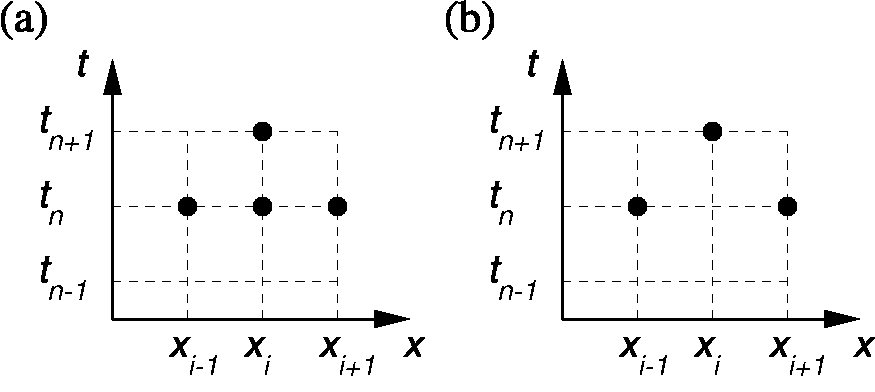
\includegraphics[height=2.5cm,width=10cm,clip=]{figures/Fig15-14top}}}
\iar stencil for FTCS (a) versus Lax-Friedrichs (b)
\pause
\bul \BFblue{hyperbolic} PDE and \BFblue{physical characteristics}
\iar the advection equation is hyperbolic as
$$ \deldelt{u} + \deldelx{\left(\underbrace{v u}_{\Blue{F}}\right)}=0 $$
and Flux Jacobian $\frac{\partial \Blue{F}}{\partial u}= v$ is real number, `characteristic speed'
\iar $x-t$ curves given by $\xi=x-vt$ yield $d\,u=0$ or $u$ constant
\ED

\end{frame}
%%%%%%%%%%%%%%%%%%%%%%%%%%%%%%%%%%%%%%%%%%%%%%%%%%%%%%%%%%%%%%%%%%%%%%%%
\begin{frame}
\frametitle{Ideal Magneto-Hydrodynamics equations}

\BD
\bul for second order wave equation
$$ \deldeltt{u}- v^2 \deldelxx{u} = 0 $$
\iar factorizes to
$$ \left(\deldelt{}- v \deldelx{}\right)\left(\deldelt{}+ v \deldelx{}\right) u = 0 $$
\iar general solution has left and right going wave with
$$ u= f(x-v t) + g(x+v t) $$
\iar initial shapes $f(x)$, $g(x)$ combine 
\iar 2 characteristics $\frac{dx}{dt}=\pm v$
\ED
\end{frame}
%%%%%%%%%%%%%%%%%%%%%%%%%%%%%%%%%%%%%%%%%%%%%%%%%%%%%%%%%%%%%%%%%%%%%%%%
\begin{frame}
\BD
\bul illustrate CFL for second order wave equation:
\hfill \\
\BFred{the domain of dependence of the differential equation should be contained in the DOD of the discretised equations} \hfill \\
\yellowbx{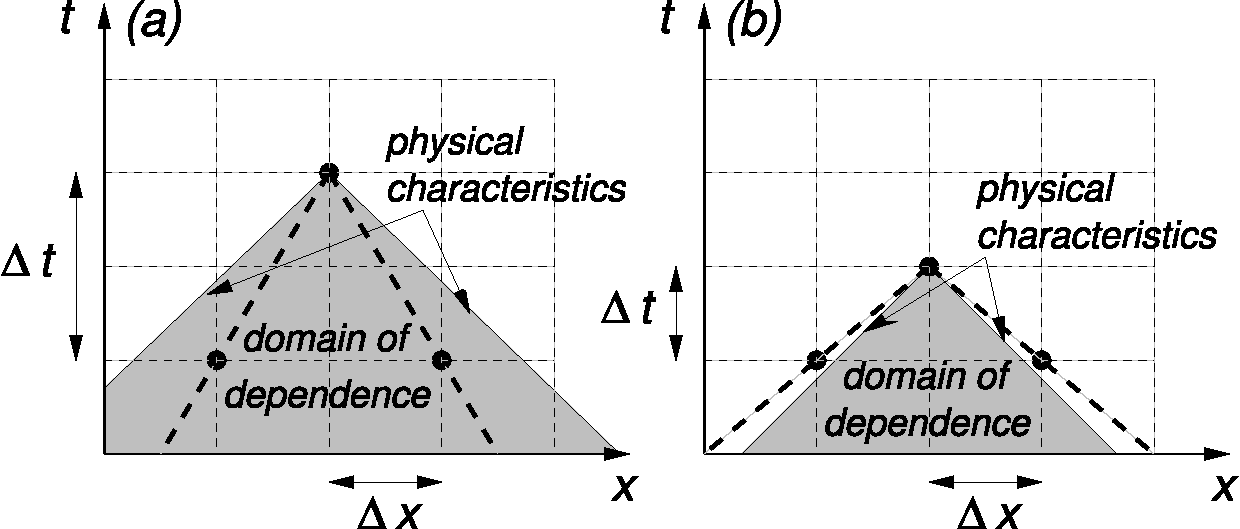
\includegraphics[height=4cm,width=10cm,clip=]{figures/Fig15-15}}
\iar stability means physical DOD contained in stencil bounds (numerical DOD), hence $\Delta t$ small enough (right case)
\pause
\bul note: linear advection $+$ wave equation: DOD only involves 1 or 2 points from $t=0$
$\leftrightarrow$ HD: DOD bounds set by $v\pm c_s$ with $c_s$ sound speed, delimits $t=0$ interval
\ED
\end{frame}
%%%%%%%%%%%%%%%%%%%%%%%%%%%%%%%%%%%%%%%%%%%%%%%%%%%%%%%%%%%%%%%%%%%%%%%%
\begin{frame}
\BD
\bul Second cure: maintain space-time symmetry of the PDE
\iar use central discretisation for both $x$ and $t$
\iar obtain \BFred{leapfrog} scheme
$$ u^{n+1}_i = u^{n-1}_i - {\Dt\over\Dx} \,(F^n_{i+1} - F^n_{i-1}) $$
\pause
\iar numerical flux function for advection is $F^n_i\equiv vu^n_i$
\iar conditionally stable and second-order accurate
\iar multiple time levels involved: $n-1$, $n$, $n+1$
\iar potential problem: even/oneven time levels may `decouple' 
\ED

\end{frame}

%%%%%%%%%%%%%%%%%%%%%%%%%%%%%%%%%%%%%%%%%%%%%%%%%%%%%%%%%%%%%%%%%%%%%%%%
\section{Hyperbolic PDE}
%%%%%%%%%%%%%%%%%%%%%%%%%%%%%%%%%%%%%%%%%%%%%%%%%%%%%%%%%%%%%%%%%%%%%%%%
\subsection{Matrix formulation of conservation laws}
%%%%%%%%%%%%%%%%%%%%%%%%%%%%%%%%%%%%%%%%%%%%%%%%%%%%%%%%%%%%%%%%%%%%%%%%
\begin{frame}
\frametitle{Flux Jacobian}

\BD
\bul von Neumann stability analysis for BTCS scheme
$$ \big|{\rm e}^{\lambda \Dt}\big| = {1 \over \left|1 + {\rm i} \frac{v \Dt}{\Dx} \sin{(k\Dx)}\right|} < 1  \qquad \hbox{for all $k$} $$
\iar \BFred{unconditionally stable}, any (large) time step $\Dt$ allowed
\vspace*{0.5cm}
\bul note: \BFblue{stability does not imply accuracy}
\iar large $\Dt$ affects accuracy, defines time resolution: behavior may involve physical timescale that needs to be resolved!
\bul implicit backward Euler: first order in time
\ED

\end{frame}
%%%%%%%%%%%%%%%%%%%%%%%%%%%%%%%%%%%%%%%%%%%%%%%%%%%%%%%%%%%%%%%%%%%%%%%%
\begin{frame}
\frametitle{Eigenvalues \& eigenvectors}

\BD
\bul von Neumann stability analysis for BTCS scheme
$$ \big|{\rm e}^{\lambda \Dt}\big| = {1 \over \left|1 + {\rm i} \frac{v \Dt}{\Dx} \sin{(k\Dx)}\right|} < 1  \qquad \hbox{for all $k$} $$
\iar \BFred{unconditionally stable}, any (large) time step $\Dt$ allowed
\vspace*{0.5cm}
\bul note: \BFblue{stability does not imply accuracy}
\iar large $\Dt$ affects accuracy, defines time resolution: behavior may involve physical timescale that needs to be resolved!
\bul implicit backward Euler: first order in time
\ED

\end{frame}
%%%%%%%%%%%%%%%%%%%%%%%%%%%%%%%%%%%%%%%%%%%%%%%%%%%%%%%%%%%%%%%%%%%%%%%%
\begin{frame}
\frametitle{Hyperbolic, parabolic and elliptic PDE}

\BD
\bul von Neumann stability analysis for BTCS scheme
$$ \big|{\rm e}^{\lambda \Dt}\big| = {1 \over \left|1 + {\rm i} \frac{v \Dt}{\Dx} \sin{(k\Dx)}\right|} < 1  \qquad \hbox{for all $k$} $$
\iar \BFred{unconditionally stable}, any (large) time step $\Dt$ allowed
\vspace*{0.5cm}
\bul note: \BFblue{stability does not imply accuracy}
\iar large $\Dt$ affects accuracy, defines time resolution: behavior may involve physical timescale that needs to be resolved!
\bul implicit backward Euler: first order in time
\ED

\end{frame}
%%%%%%%%%%%%%%%%%%%%%%%%%%%%%%%%%%%%%%%%%%%%%%%%%%%%%%%%%%%%%%%%%%%%%%%%
\begin{frame}
\frametitle{Linear, non-linear \& quasi-linear}

\BD
\bul von Neumann stability analysis for BTCS scheme
$$ \big|{\rm e}^{\lambda \Dt}\big| = {1 \over \left|1 + {\rm i} \frac{v \Dt}{\Dx} \sin{(k\Dx)}\right|} < 1  \qquad \hbox{for all $k$} $$
\iar \BFred{unconditionally stable}, any (large) time step $\Dt$ allowed
\vspace*{0.5cm}
\bul note: \BFblue{stability does not imply accuracy}
\iar large $\Dt$ affects accuracy, defines time resolution: behavior may involve physical timescale that needs to be resolved!
\bul implicit backward Euler: first order in time
\ED

\end{frame}
%%%%%%%%%%%%%%%%%%%%%%%%%%%%%%%%%%%%%%%%%%%%%%%%%%%%%%%%%%%%%%%%%%%%%%%%
\subsection{Time advance}
%%%%%%%%%%%%%%%%%%%%%%%%%%%%%%%%%%%%%%%%%%%%%%%%%%%%%%%%%%%%%%%%%%%%%%%%
\begin{frame}
\frametitle{Explicit}

\BD
\bul spatial differences as average of $n$-th and $(n+1)$-th time step
$$  u^{n+1}_i = u^n_i - \onefourth v \,{\Dt \over \Dx} \,(u^{\Red{n+1}}_{i+1}+ u^{\Red{n}}_{i+1} - u^{\Red{n+1}}_{i-1} - u^{\Red{n}}_{i-1})  $$
\iar second order \BFred{Crank--Nicolson method}
\iar \BFblue{Exercise}: show that this scheme is unconditionally stable, 2nd order accurate
\vspace*{0.5cm}
\bul stencils for BTCS (left) and Crank-Nicolson (right) \hfill \\
\centerline{\yellowbx{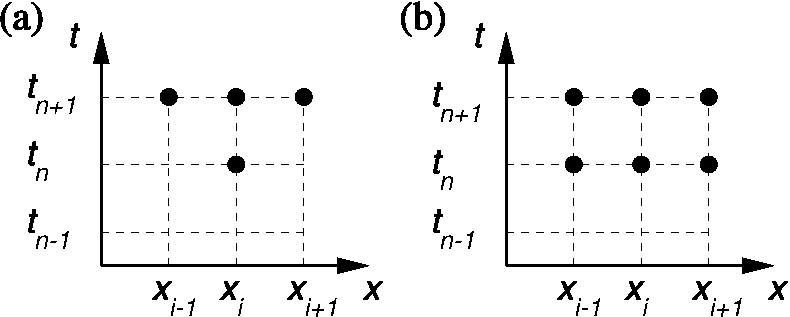
\includegraphics[height=3cm]{figures/Fig15-17}}}
\ED

\end{frame}
%%%%%%%%%%%%%%%%%%%%%%%%%%%%%%%%%%%%%%%%%%%%%%%%%%%%%%%%%%%%%%%%%%%%%%%%
\begin{frame}
\frametitle{Implicit}

\BD
\bul spatial differences as average of $n$-th and $(n+1)$-th time step
$$  u^{n+1}_i = u^n_i - \onefourth v \,{\Dt \over \Dx} \,(u^{\Red{n+1}}_{i+1}+ u^{\Red{n}}_{i+1} - u^{\Red{n+1}}_{i-1} - u^{\Red{n}}_{i-1})  $$
\iar second order \BFred{Crank--Nicolson method}
\iar \BFblue{Exercise}: show that this scheme is unconditionally stable, 2nd order accurate
\vspace*{0.5cm}
\bul stencils for BTCS (left) and Crank-Nicolson (right) \hfill \\
\centerline{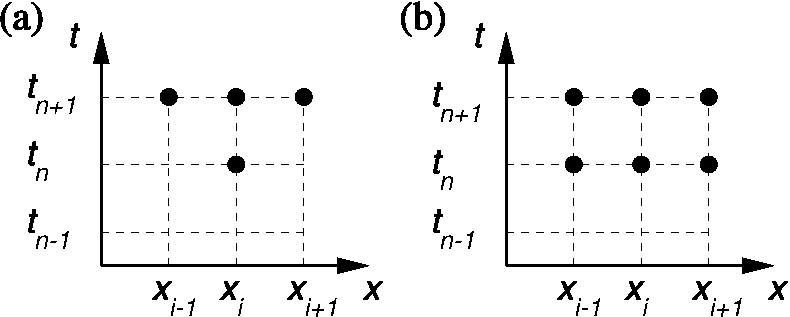
\includegraphics[height=3cm]{figures/Fig15-17}}
\ED

\end{frame}
%%%%%%%%%%%%%%%%%%%%%%%%%%%%%%%%%%%%%%%%%%%%%%%%%%%%%%%%%%%%%%%%%%%%%%%%
\subsection{Linear advective equations}
%%%%%%%%%%%%%%%%%%%%%%%%%%%%%%%%%%%%%%%%%%%%%%%%%%%%%%%%%%%%%%%%%%%%%%%%
\begin{frame}
\frametitle{Properties}
\BD
\bul many practical implementations use `method of lines'
\iar vector $\bfu$ of unknowns after first spatial discretization
\iar obtain ODE system
$$ \ddt{\bfu}=\bff(\bfu) $$
\iar RHS vector function $\bff$ could even be nonlinear in $\bfu$
\vspace*{0.5cm}
\bul discretize ODE in time using parameter $\alpha$ in
$$ \bfu^{n+1}=\bfu^n+\Dt\left[\alpha\bff(\bfu^{n+1}) + (1-\alpha)\bff(\bfu^n)\right] $$
\iar note case $\alpha=0$: explicit (unstable) forward Euler method
\ED

\end{frame}
%%%%%%%%%%%%%%%%%%%%%%%%%%%%%%%%%%%%%%%%%%%%%%%%%%%%%%%%%%%%%%%%%%%%%%%%
\begin{frame}
\frametitle{Characteristics}
\BD
\bul many practical implementations use `method of lines'
\iar vector $\bfu$ of unknowns after first spatial discretization
\iar obtain ODE system
$$ \ddt{\bfu}=\bff(\bfu) $$
\iar RHS vector function $\bff$ could even be nonlinear in $\bfu$
\vspace*{0.5cm}
\bul discretize ODE in time using parameter $\alpha$ in
$$ \bfu^{n+1}=\bfu^n+\Dt\left[\alpha\bff(\bfu^{n+1}) + (1-\alpha)\bff(\bfu^n)\right] $$
\iar note case $\alpha=0$: explicit (unstable) forward Euler method
\ED

\end{frame}
%%%%%%%%%%%%%%%%%%%%%%%%%%%%%%%%%%%%%%%%%%%%%%%%%%%%%%%%%%%%%%%%%%%%%%%%
\begin{frame}
\frametitle{Stencils, domain of dependence, range of influence}
\BD
\bul many practical implementations use `method of lines'
\iar vector $\bfu$ of unknowns after first spatial discretization
\iar obtain ODE system
$$ \ddt{\bfu}=\bff(\bfu) $$
\iar RHS vector function $\bff$ could even be nonlinear in $\bfu$
\vspace*{0.5cm}
\bul discretize ODE in time using parameter $\alpha$ in
$$ \bfu^{n+1}=\bfu^n+\Dt\left[\alpha\bff(\bfu^{n+1}) + (1-\alpha)\bff(\bfu^n)\right] $$
\iar note case $\alpha=0$: explicit (unstable) forward Euler method
\ED

\end{frame}
%%%%%%%%%%%%%%%%%%%%%%%%%%%%%%%%%%%%%%%%%%%%%%%%%%%%%%%%%%%%%%%%%%%%%%%%
\subsection{The Riemann problem}
%%%%%%%%%%%%%%%%%%%%%%%%%%%%%%%%%%%%%%%%%%%%%%%%%%%%%%%%%%%%%%%%%%%%%%%%
\begin{frame}
\frametitle{The Riemann problem}
$$ \bfu^{n+1}=\bfu^n+\Dt\left[\alpha\bff(\bfu^{n+1}) + (1-\alpha)\bff(\bfu^n)\right] $$
\BD
\bul $\alpha=1$ is \BF{implicit backward Euler}
\bul $\alpha=1/2$ gives second-order accuracy, \BFblue{trapezoidal method}
\iar Crank-Nicolson for central discretization of flux in $\bff$
\vspace*{0.5cm}
\bul when $\bff$ nonlinear: linearize using
$$ \bff(\bfu^{n+1}) \approx \bff(\bfu^n) + {\partial \bff^n \over \partial \bfu} \,(\bfu^{n+1} - \bfu^n) $$
\iar introduces matrix  $\displaystyle {\partial \bff^n \over \partial \bfu}$ called \BFred{\em ``Jacobian matrix''} of $\bff$
\ED
\end{frame}
%%%%%%%%%%%%%%%%%%%%%%%%%%%%%%%%%%%%%%%%%%%%%%%%%%%%%%%%%%%%%%%%%%%%%%%%
\end{document}
